% easychair.tex,v 3.5 2017/03/15

\documentclass{easychair}
%\documentclass[EPiC]{easychair}
%\documentclass[EPiCempty]{easychair}
%\documentclass[debug]{easychair}
%\documentclass[verbose]{easychair}
%\documentclass[notimes]{easychair}
%\documentclass[withtimes]{easychair}
%\documentclass[a4paper]{easychair}
%\documentclass[letterpaper]{easychair}

\usepackage{doc}

% use this if you have a long article and want to create an index
% \usepackage{makeidx}

% In order to save space or manage large tables or figures in a
% landcape-like text, you can use the rotating and pdflscape
% packages. Uncomment the desired from the below.
%
% \usepackage{rotating}
% \usepackage{pdflscape}

% Some of our commands for this guide.
%
\newcommand{\easychair}{\textsf{easychair}}
\newcommand{\miktex}{MiK{\TeX}}
\newcommand{\texniccenter}{{\TeX}nicCenter}
\newcommand{\makefile}{\texttt{Makefile}}
\newcommand{\latexeditor}{LEd}

%\makeindex

%% Front Matter
%%
% Regular title as in the article class.
%
\title{The {\easychair} Class File\\
       Documentation and Guide for Authors%
\thanks{Other people who contributed to this document include Maria Voronkov
  (Imperial College and EasyChair) and Graham Gough (The University of
  Manchester).}}

% Authors are joined by \and. Their affiliations are given by \inst, which indexes
% into the list defined using \institute
%
\author{
Serguei A. Mokhov\inst{1}\thanks{Designed and implemented the class style}
\and
    Geoff Sutcliffe\inst{2}\thanks{Did numerous tests and provided a lot of suggestions}
\and
   Andrei Voronkov\inst{3}\inst{4}\inst{5}\thanks{Masterminded EasyChair and created versions
     3.0--3.5 of the class style}
}

% Institutes for affiliations are also joined by \and,
\institute{
  Concordia University,
  Montreal, Quebec, Canada\\
  \email{mokhov@cse.concordia.ca}
\and
   University of Miami,
   Miami, Florida, U.S.A.\\
   \email{geoff@cs.miami.edu}\\
\and
   University of Manchester,
   Manchester, U.K.\\
   \email{andrei@voronkov.com}\\
\and
   Chalmers University of Technology,
   Gothenburg, Sweden
\and
   EasyChair
 }

%  \authorrunning{} has to be set for the shorter version of the authors' names;
% otherwise a warning will be rendered in the running heads. When processed by
% EasyChair, this command is mandatory: a document without \authorrunning
% will be rejected by EasyChair

\authorrunning{Mokhov, Sutcliffe and Voronkov}

% \titlerunning{} has to be set to either the main title or its shorter
% version for the running heads. When processed by
% EasyChair, this command is mandatory: a document without \titlerunning
% will be rejected by EasyChair
\titlerunning{The {\easychair} Class File}

\begin{document}

\maketitle

\begin{abstract}
  In order to ease the lives of authors, editors, and trees, we present an
  easy-to-read guide to the easy-to-use {\easychair} {\LaTeX2e} document style
  class for EasyChair-based electronic and on-paper publishing of workshop and conference
  proceedings.
\end{abstract}

% The table of contents below is added for your convenience. Please do not use
% the table of contents if you are preparing your paper for publication in the
% EPiC Series or Kalpa Publications series

\setcounter{tocdepth}{2}
{\small
\tableofcontents}

%\section{To mention}
%
%Processing in EasyChair - number of pages.
%
%Examples of how EasyChair processes papers. Caveats (replacement of EC
%class, errors).

%------------------------------------------------------------------------------
\section{Introduction}
\label{sect:introduction}

The {\easychair} class was designed to be easy to use, and specifically favors
electronic and on-paper publishing by the EasyChair conference system
\cite{easychair}, including the
\href{http://www.easychair.org/publications/EPiC}{EasyChair EPiC
  Series} and \href{http://www.easychair.org/publications/Kalpa}{EasyChair Kalpa
  Publications}. 
EasyChair is a free conference management system that is flexible, easy to use,
and has many features to make it suitable for various conference models. It is
currently probably the most commonly used conference management system
\cite{easychair}.  

The {\easychair} class was designed according to some requirements, which
are described in Appendix~\ref{sect:easychair-requirements}. 
An article that occupies approximately 15 LNCS-formatted pages
takes up approximately 14 {\easychair} pages.

\begin{figure}[tb]
	\begin{centering}
	
\includegraphics[width=0.5\textwidth]{logoEC}
	\caption{EasyChair logo}
	\label{fig:easychair-logo}
	\end{centering}
\end{figure}

%------------------------------------------------------------------------------
\section{Typesetting}
\label{sect:typesetting}

Typesetting with {\easychair} is, well, easy.  Just by using the
document class entry in the document's preamble as follows:
\verb+\documentclass{easychair}+ the typesetting work is nearly done.
The {\easychair} class is a relatively conservative extension of the
standard \texttt{article} class, so most of the environments, section
headers, etc. defined by \texttt{article} are available.

%------------------------------------------------------------------------------
\subsection{Generalities}
\label{sect:generalities}

The following are the general default parameters {\easychair}
introduces into the typesetting aspect of articles. If you use
\easychair\ for proceedings or other kinds of publishing through
EasyChair, do not alter these -- papers deviating from the formatting
standards will be rejected by EasyChair.

\begin{enumerate}
\item
The default paper size is US letter. It can be explicitly set to A4 
(\texttt{a4paper}) or letter (\texttt{letterpaper}) paper in the
document class entry, e.g.:\\\verb+\documentclass[a4paper]{easychair}+

\item
The print area for both letter and A4 paper sizes is 145x224 mm. This size
has been selected to allow for inexpensive printing using our current
print-on-demand publisher.

\item
The base font is Computer Modern. The base font size is 10pt. If you
use any other font size, there is no guarantee that the produced
document will look nice or fit into our standard page size.

\item
The references list is condensed. The default bibliography styles, such as
\texttt{plain}, \texttt{abbrv}, and \texttt{alpha}, are suggested.

\item
PNG, JPG, and PDF images are supported, i.e., those that are supported
by the standard \texttt{graphicx} package \cite{graphicx-package}, and
render nicely in online versions of PDF documents.  This document
shows some examples of JPG and PDF images, for example in
Figure~\ref{fig:easychair-logo}. If the papers are designed for
publishing in print, the images should be at least 300dpi in
resolution. 

\end{enumerate}

%------------------------------------------------------------------------------
\subsection{Front Matter}
\label{sect:front-matter}

The front matter of an {\easychair} article follows the \texttt{article}
style, augmented with the \verb+\titlerunning+ and \verb+\authorrunning+
commands for use by authors. 
For the \verb+\author+ command with multiple authors, use \verb+\and+ to
separate authors from different institutions, as done in this document.
Institutions are defined using \verb+\institute+ in a similar way and affiliations of authors assigned using \verb+\inst+.
Authors must set the \verb+\titlerunning+ and \verb+\authorrunning+.
For example, the front matter of this document defined the authors
and title as follows:

%---------------------------------------------------------------

\noindent\small
\begin{verbatim}
\title{The {\easychair} Class File\\
       Documentation and Guide for Authors%
\thanks{Other people who contributed to this document include Maria Voronkov
  (Imperial College and EasyChair) and Graham Gough (The University of
  Manchester).}}

% Authors are joined by \and. Their affiliations are given by \inst, which indexes
% into the list defined using \institute
%
\author{
Serguei A. Mokhov\inst{1}\thanks{Designed and implemented the class style}
\and
   Geoff Sutcliffe\inst{2}\thanks{Did numerous tests and provided a lot of suggestions}
\and
   Andrei Voronkov\inst{3}\inst{4}\inst{5}\thanks{Masterminded EasyChair and created 
     versions 3.0--3.5 of the class style}
}

% Institutes for affiliations are also joined by \and,
\institute{
  Concordia University,
  Montreal, Quebec, Canada\\
  \email{mokhov@cse.concordia.ca}
\and
   University of Miami,
   Miami, Florida, U.S.A.\\
   \email{geoff@cs.miami.edu}\\
\and
   University of Manchester,
   Manchester, U.K.\\
   \email{andrei@voronkov.com}\\
\and
   Chalmers University of Technology,
   Gothenburg, Sweden
\and
   EasyChair
 }

\authorrunning{Mokhov, Sutcliffe and Voronkov}
\titlerunning{The {\easychair} Class File}
\end{verbatim}
\normalsize

%------------------------------------------------------------------------------
\subsection{Page Numbering}
\label{sect:page-numbering}

Page numbers are at the bottom of every page. Authors must leave the
page numbers in as-is. When EasyChair proceedings and Procedia volumes are processed by
EasyChair, the correct volume page numbers will be inserted
automatically.

%------------------------------------------------------------------------------
\subsection{Section Headings and Capitalization}
\label{sect:section-headings}

Section and paragraph headings in {\easychair} are invoked via the standard 
commands, such as
\verb+\section+,
\verb+\subsection+,
\verb+\subsubsection+, and
\verb+\paragraph+.
Generally, every non-trivial word in a heading must be capitalized according to
general capitalization guidelines. A reasonable rule to use is that
all prepositions, coordinating conjunctions and articles having four
or fewer letters should not be capitalized. If you do not know what it
means, simply do not capitalize the following words:
\textit{amid, anti, as, at, atop, but, by, down, for, from, in, into, like,
near, next, of, off, on, onto, out, over, pace, past, per, plus, qua,
save, than, till, to, up, upon, via, with, for, and, nor, but, or,
yet, so, a, an, the.} For example, if you want to call your paper
``oldest but goldest'', then the proper title for it is ``Oldest but
Goldest''. ``Oldest but goldest'' is wrong (since ``goldest'' is not
capitalized) and ``Oldest But Goldest'' is wrong (``but'' should stay
lower-cased since it belongs to the list of words above.) Needless to
say, ``OLDEST BUT GOLDEST'' is very wrong.

Paragraph headings should not be capitalized and should have a
trailing period. That is, you should write

\begin{quote}
\verb|\paragraph{EasyChair is cool.}|
\end{quote}
rather than 

\begin{quote}
\verb|\paragraph{EasyChair is cool}|
\end{quote}
unless your aim was to write something like

\begin{quote}
\verb|\paragraph{EasyChair is cool} when you use it for publishing.| 
\end{quote}
Of course, you are welcome to replace the trailing period by any other
punctuation mark, for example 

\begin{quote}
\verb|\paragraph{EasyChair is cool!}|
\end{quote}

See the examples in this document, e.g.,
Section~\ref{sect:typesetting} is a section, this 
(Section~\ref{sect:section-headings}) is a subsection, and
Section~\ref{sect:subsubsection-headings} is a subsubsection.

%------------------------------------------------------------------------------
\subsubsection{Subsubsection Header}
\label{sect:subsubsection-headings}

This is a subsubsection. 

\paragraph{Paragraph header.}

This is a paragraph. 
One way of saving space when hyper-references are not essential is to 
use paragraphs instead of subsubsections.

%------------------------------------------------------------------------------
\subsection{Mathematics}
\label{sect:mathematics}

Mathematics can be done inline for simple things, e.g., an equation
$x = 0$, possibly with super and subscripts, e.g., $x^2_k \approx 27$,
Greek letters, e.g., $\alpha \cup \Theta \ne \gamma$, etc.
Larger formulae must be done using {\tt \verb|\|[}~~{\tt \verb|\|]}
bracketing, e.g.,
\[
\int_{0}^{1} x dx = \left[ \frac{1}{2}x^2 \right]_{0}^{1} = \frac{1}{2}
\]
or using {\tt \verb|\|begin\{equation\}} and {\tt \verb|\|end\{equation\}} for
numbered equations, e.g.,
\begin{equation}
e^x = \sum_{n=0}^\infty \frac{x^n}{n!} = \lim_{n\rightarrow\infty} (1+x/n)^n
\end{equation}

Use {\tt \verb|\|begin\{align*\}} and {\tt \verb|\|end\{align*\}} (or without
the {\tt *} include number) to align equations, e.g.,
\begin{align*}
x^2 + y^2 &= 1 \\
y &= \sqrt{1 - x^2}
\end{align*}

Fonts, using \verb|\matcal| and others can also be used in the math mode: $\mathcal{ALC}$.

%------------------------------------------------------------------------------
\subsection{Tables}
\label{sect:tables}

Table~\ref{tab:ltbexample} shows an example of a table of data that was
conveniently available (i.e., the data has nothing to do with
{\easychair}) apart from being related to the research of two of its
authors. 

\begin{table}[htp]
	\begin{centering}
		\begin{tabular}{lrrrrrrrr}
		\hline
		ATP System            & LTB & Avg  &Prfs & SOTA & \multicolumn{1}{c}{$\mu$} & CYC & MZR & SMO \\
		                      & /100& time & out & Con. & Eff. & /35 & /40 & /25 \\
		\hline
		Vampire-LTB 11.0      &  69 & 24.5 &  69 & 0.37 & 28.1 &  23 &  22 &  24 \\
		iProver-SInE 0.7      &  67 & 76.5 &   0 & 0.36 &  8.8 &  28 &  14 &  25 \\
		SInE 0.4              &  64 & 75.3 &  64 & 0.32 &  8.5 &  26 &  13 &  25 \\
		leanCoP-SInE 2.1      &  35 &110.8 &  35 & 0.23 &  3.2 &  23 &   1 &  11 \\
		E-LTB 1.1pre          &  18 & 63.4 &   0 & 0.21 &  2.8 &   7 &   9 &   2 \\
		EP-LTB 1.1pre         &  18 & 77.8 &  18 & 0.21 &  2.3 &   7 &   9 &   2 \\
		E-KRH'-LTB 1.1.3      &   0 &   -- &  -- &   -- &   -- &   0 &   0 &   0 \\
		\hline
		\end{tabular}
		\caption{LTB division results}
		\label{tab:ltbexample}
	\end{centering}
\end{table}

%------------------------------------------------------------------------------
\subsection{References}
\label{sect:references}

References must be provided in a {\tt .bib} file, so that \BibTeX\ can
be used to generate the references in a consistent style in a volume.
The preferred styles are {\tt plain} and {\tt alpha}.
For example, the references for this paper are generated from the
lines
\begin{verbatim}
    \bibliographystyle{plain}
    \bibliography{easychair}
\end{verbatim}
and a way to compose the entires, e.g. citing this class style~\cite{easychair-latex-class}
is below:
\small
\begin{verbatim}
    @misc
    {
      easychair-latex-class,
      author       = {Serguei A. Mokhov and Geoff Sutcliffe and Andrei Voronkov},
      title        = {The {\sf easychair} Class File Documentation and Guide
                      for Authors},
      year         = {2008--2011},
      howpublished = {[online]},
      note         = {Available at \url{http://easychair.org/easychair.zip}}
    }
\end{verbatim}
\normalsize

%------------------------------------------------------------------------------
\section{Installation and Usage Instructions}
\label{sect:installation-usage}

%------------------------------------------------------------------------------
\subsection{Installation}

The ``installation'' of the {\easychair} document class is easy.
Download the latest version of the \texttt{easychair.zip} package 
from \url{http://www.easychair.org/easychair.zip}
and unzip it in the directory where you will prepare your paper.
You will get the following files, out of which you may need to keep only 
the \texttt{easychair.cls} style class if you are familiar with the rest 
of the files and do not require them to get started.
We are also working to make {\easychair} available from CTAN \cite{ctan},
such that it can be installed with the popular \TeX Live \cite{texlive} and
{\miktex} \cite{miktex} \LaTeX\ package management systems.

\begin{itemize}
\item
\texttt{easychair.cls} -- the class file that this is all about.

\item
\texttt{easychair-a4.pdf} -- the PDF version of this guide rendered using 
\texttt{a4paper} option.

\item
\texttt{easychair.tex} -- the {\LaTeX} source of this guide, 
and
\texttt{easychair.bib} -- the supporting bibliography entries found starting 
on page~\pageref{sect:bib}.

\item
\texttt{logoEC.pdf} -- the PDF version of the EasyChair logo rendered in
Figure~\ref{fig:easychair-logo} and
\texttt{throneEC.jpg} -- the JPG version of the easy throne rendered in 
Figure~\ref{fig:easythrone}.

\end{itemize}

%------------------------------------------------------------------------------
\subsection{Required Packages}

The {\easychair} class relies only on packages deemed standard and shipped by
most {\LaTeX} distributions in the worlds of Linux (current \texttt{texlive} \cite{texlive}
or older \texttt{tetex}), MacOS X,
and Windows (via Cygwin or {\miktex}).
If for some reason your distribution is old or doesn't have the packages
listed below, you can always obtain a copy from CTAN \cite{ctan}. Note
that EasyChair loads this packages automatically so you don't have to
use \verb|\usepackage| to use any of these packages.

\begin{itemize}
\item
\texttt{url} \cite{url-package} (included also by \texttt{hyperref} automatically) -- to provide URL rendering support for the
monospaced font, which takes care of special characters as well as line 
wrapping.

\item
\texttt{hyperref} \cite{hyperref-package} -- to allow hyperlinking of URLs and
cross references within an article.
Its options are set to either \verb+letterpaper+ or \verb+a4paper+, depending
on the \verb+\documentclass+ options.

\item
\texttt{graphicx} \cite{graphicx-package} -- the standard package for rendering
PNG, JPG, and PDF graphic images, primarily in \texttt{figure} environments.

\item
optional \texttt{mathptmx} \cite{mathptmx-package} -- Times base font for compactness
(use with the \texttt{withtimes} {\easychair} option).

\item
\texttt{listings} \cite{listings-package} -- to allow highlighted source code 
listing styles.

\item
\texttt{latexsym} \cite{latexsym-package} -- to provide common math and other 
symbols.

\item
\texttt{amsthm} \cite{amsthm-package} -- to provide {\AmS} theorem-like 
environments.

\item
\texttt{empheq} \cite{empheq-package} -- to provide equation environments, etc.

\item
\texttt{geometry} \cite{geometry-package} -- to set {\easychair} margins, 
outlined in Section~\ref{sect:generalities}.

\item
\texttt{lastpage} \cite{lastpage-package} -- to allow computationally
referencing the last page.

\item
\texttt{fancyhdr} \cite{fancyhdr-package} -- for running heads.

\item
\texttt{footmisc} \cite{footmisc-package} -- to ensure that footnotes are
always at the bottom.

\item
optional \texttt{makeidx} \cite{makeidx-package} -- for index generation
(use with the \texttt{thesis} {\easychair} option).

\item
\texttt{eso-pic} \cite{eso-pic-package} -- for draft versions and checking page
overlflows vs. a border drawn around the headers, footers, and the main body of
the article.

\end{itemize}

%------------------------------------------------------------------------------
\subsection{Recommended Packages}
\label{sect:recommended-packages}

Here is a list of some packages that this guide's authors have experimented 
with, and which are suitable for inclusion if needed by article authors.
These packages must be loaded using \verb+\usepackage+.
In general, authors may use any standard packages provided they do not change
the basic layout and font settings established by the {\easychair} class.
Such packages must be provided with the submission of articles.

\begin{itemize}
\item
\texttt{rotating} \cite{rotating-package} -- to rotate floats (figures and
tables) on the page, when wide tables or figures do not fit in portrait layout.

\item
\texttt{pdflscape} \cite{pdflscape-package} -- similar to \texttt{rotating}, 
but also allows rotating text to make it conveniently viewable in a PDF 
viewer that supports individual rotated pages.
A possible disadvantage is that a page break is forced, which may create
gaps before or after the landscape page.

\item
\texttt{algorithm2e} \cite{algorithm2e-package} -- provides a figure-like
algorithm environment for formal algorithm presentation with highlighting.

\end{itemize}

%------------------------------------------------------------------------------
\subsection{Compiling}
\label{sect:compiling}

\texttt{pdflatex} \cite{pdflatex-instructions} is the preferred tool for
producing PDF files with {\easychair} class documents.
The author kit (\texttt{easychair.zip}) includes some minimal automation 
that authors can use at their discretion.

\begin{itemize}
\item
Linux and UNIX-like platforms (also works under Cygwin and MacOS X):
A {\makefile} is provided for the GNU \texttt{make} \cite{gmake} utility,
so this document can be compiled by typing \texttt{make} at the terminal 
prompt (on the systems where both GNU and non-GNU versions of \texttt{make} 
are installed, one may need to use \texttt{gmake}).

\item
Microsoft Windows:
{\texniccenter} \cite{texniccenter} or {\latexeditor} \cite{led} and
{\miktex} \cite{miktex} as their backend are common tools
for {\LaTeX} processing under Microsoft Windows. 
The former provide a GUI front-end to {\LaTeX}, and the latter is the 
Windows native-compiled binaries and standard packages with 
a comprehensive package update tool. 
The \texttt{easychair.tcp} project file is provided for {\texniccenter} users,
as well as \texttt{easychair.lpr} for {\latexeditor} users.

\item
MacOS X:
TeXShop \cite{texshop} is a tool for {\LaTeX} processing under Mac OS X.
It provides a GUI front-end to {\LaTeX}. The backend can be installed
through the \texttt{fink} \cite{fink} repository or the Darwin Ports.
\end{itemize}

Some authors use packages that require the use of \texttt{latex}
instead of \texttt{pdflatex}, most notably \texttt{pstricks} and its
derivatives. If switching to modern packages, such as
\texttt{tikz} is not an option, these authors can use the {\easychair}
class with \texttt{latex}. 

%------------------------------------------------------------------------------
\subsection{Bug Reports}
\label{sec:bug-reports}

Please report bugs, errors, and omissions you find with the {\easychair} 
class to its current maintainer, Andrei Voronkov,
at \url{andrei@voronkov.com}. Any \emph{constructive} feedback is
always welcome. If anybody has a very hard question, we might be
unable to answer it without Sergei. If anybody knows his whereabouts,
Geoff and Andrei have the ransom money ready.

%------------------------------------------------------------------------------

\section{Avoiding Text Overflows}

When used in EasyChair, the {\easychair} class is intended for
publishing, including printing. This implies that the text of your
document should not overflow the page dimensions. This section gives
some practical advice on how you can avoid text overflows. When you
run \texttt{pdflatex} or \texttt{latex} on your files, you sometimes
get warnings like

\small
\begin{verbatim}
  LaTeX Warning: Overfull \hbox (7.43138pt too wide) in paragraph at lines 994--994
\end{verbatim}
\normalsize
or

\small
\begin{verbatim}
  LaTeX Warning: Float too large for page by 55.21666pt on input line 638.
\end{verbatim}
\normalsize
They mean what they say: your text overflows the allowed space. When
you prepare a PDF document that will only be used online or as a
draft, in many cases you can ignore these warnings, since they only
make your document uglier than it could be but it remains still
readable. However, for documents that are supposed to be printed,
overflows make a lot of difference. There is no universal recipe on
how to make your text fit into the page. However, there are some
common cases that can be easily fixed using the tricks described
here. 

\subsection{Using the \texttt{debug} Option to Check for Overflows}

A general guideline is that you should first check how the alleged
overflows looks in reality. For example, some LaTeX overflows are
invisible or hardly noticeable for people and overlows by
less than 4pt look OK anyhow. The {\easychair} class has an option
\texttt{debug} that adds to each page of your documents a red frame
corresponding to the allowed page
dimensions. Figure~\ref{fig:redframe} on page~\pageref{fig:redframe}
shows an example of a page created using this style. With such a red
frame, you can clearly see any overflows apart from very minor ones.


\begin{figure}
  \begin{centering}
    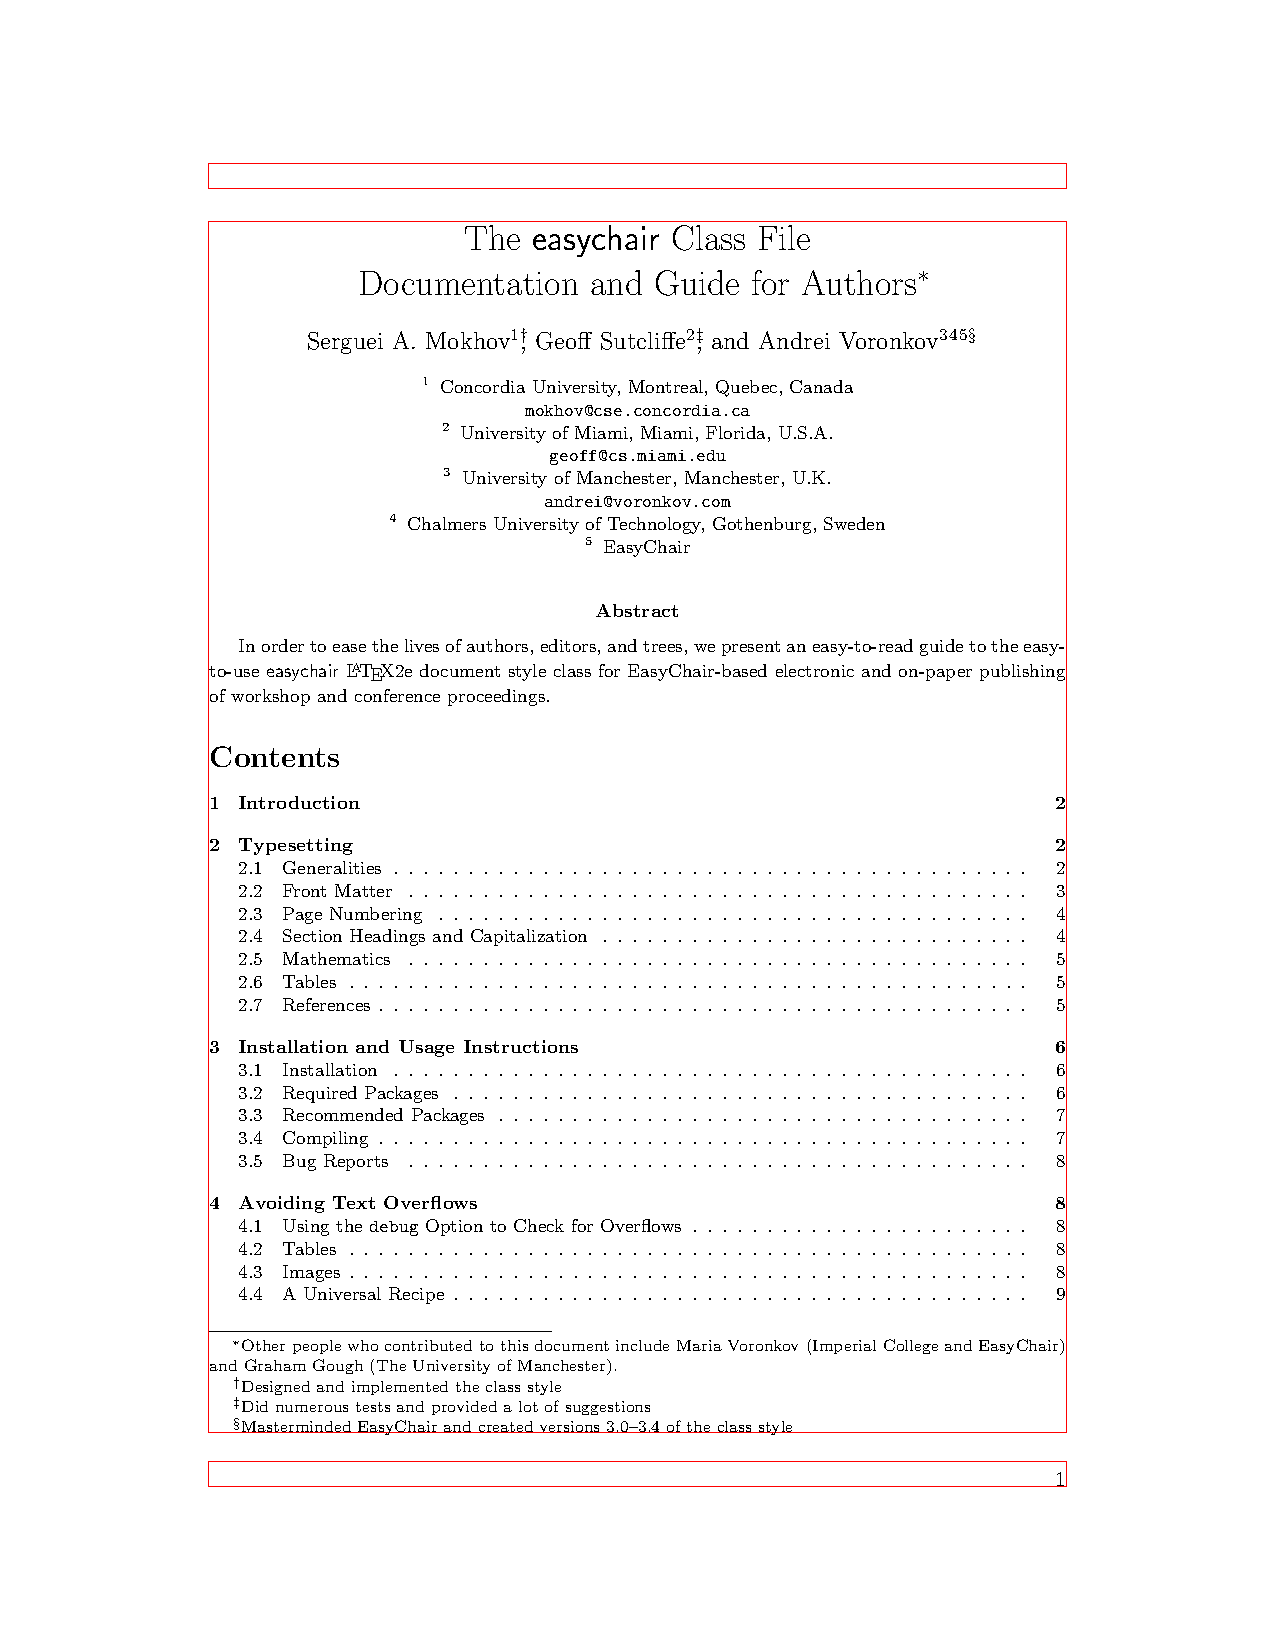
\includegraphics[width=0.89\textwidth]{debug.pdf}
    \caption{A page of a document created using the \texttt{debug}
      option} 
    \label{fig:redframe}
  \end{centering}
\end{figure}

\subsection{Tables}

Many page overflows happen because of large tables. In many case these
overflows can be easily removed by slightly reducing padding added by
\LaTeX\ to every column. It is controlled by the \LaTeX\ command
\verb|\tabcolsep| whose value by default is 6pt. Even small changes in
the value of this command may give drastic reductions in the width of
tables. This is illustrated in Figure~\ref{fig:tabcolsep} on
page~\pageref{fig:tabcolsep}. Note though that there is no free lunch:
smaller values for this command may result in lower redability.

%------------------------------------------------------------
\begin{figure}[tb]\small
\begin{center}
  \begin{tabular}{lrrrrrrrr}
    \hline
    ATP System            & LTB & Avg  &Prfs & SOTA & \multicolumn{1}{c}{$\mu$} & CYC & MZR & SMO \\
   \hline
    Vampire-LTB 11.0      &  69 & 24.5 &  69 & 0.37 & 28.1 &  23 &  22 &  24 \\
    iProver-SInE 0.7      &  67 & 76.5 &   0 & 0.36 &  8.8 &  28 &  14 &  25 \\
   \hline
  \end{tabular}
\end{center}

\begin{center}\renewcommand{\tabcolsep}{5pt}
  \begin{tabular}{lrrrrrrrr}
    \hline
    ATP System            & LTB & Avg  &Prfs & SOTA & \multicolumn{1}{c}{$\mu$} & CYC & MZR & SMO \\
   \hline
    Vampire-LTB 11.0      &  69 & 24.5 &  69 & 0.37 & 28.1 &  23 &  22 &  24 \\
    iProver-SInE 0.7      &  67 & 76.5 &   0 & 0.36 &  8.8 &  28 &  14 &  25 \\
   \hline
  \end{tabular}
\end{center}

\begin{center}\renewcommand{\tabcolsep}{3pt}
  \begin{tabular}{lrrrrrrrr}
    \hline
    ATP System            & LTB & Avg  &Prfs & SOTA & \multicolumn{1}{c}{$\mu$} & CYC & MZR & SMO \\
   \hline
    Vampire-LTB 11.0      &  69 & 24.5 &  69 & 0.37 & 28.1 &  23 &  22 &  24 \\
    iProver-SInE 0.7      &  67 & 76.5 &   0 & 0.36 &  8.8 &  28 &  14 &  25 \\
   \hline
  \end{tabular}
\end{center}

\begin{center}\renewcommand{\tabcolsep}{1pt}
  \begin{tabular}{lrrrrrrrr}
    \hline
    ATP System            & LTB & Avg  &Prfs & SOTA & \multicolumn{1}{c}{$\mu$} & CYC & MZR & SMO \\
   \hline
    Vampire-LTB 11.0      &  69 & 24.5 &  69 & 0.37 & 28.1 &  23 &  22 &  24 \\
    iProver-SInE 0.7      &  67 & 76.5 &   0 & 0.36 &  8.8 &  28 &  14 &  25 \\
   \hline
  \end{tabular}
\end{center}
\normalsize

\caption{Original table and tables with \texttt{tabcolsep} set to 5pt,
  3pt, and 1pt
  \label{fig:tabcolsep}}

\end{figure}
%------------------------------------------------------------

\subsection{Images}

Images included using \verb|\includegraphics| are easy to resize since
one can specify the size of the result explicitly. For example,
Figure~\ref{fig:easythrone} shows three copies of the same image
having different sizes obtained using the following commands:

\begin{verbatim}
  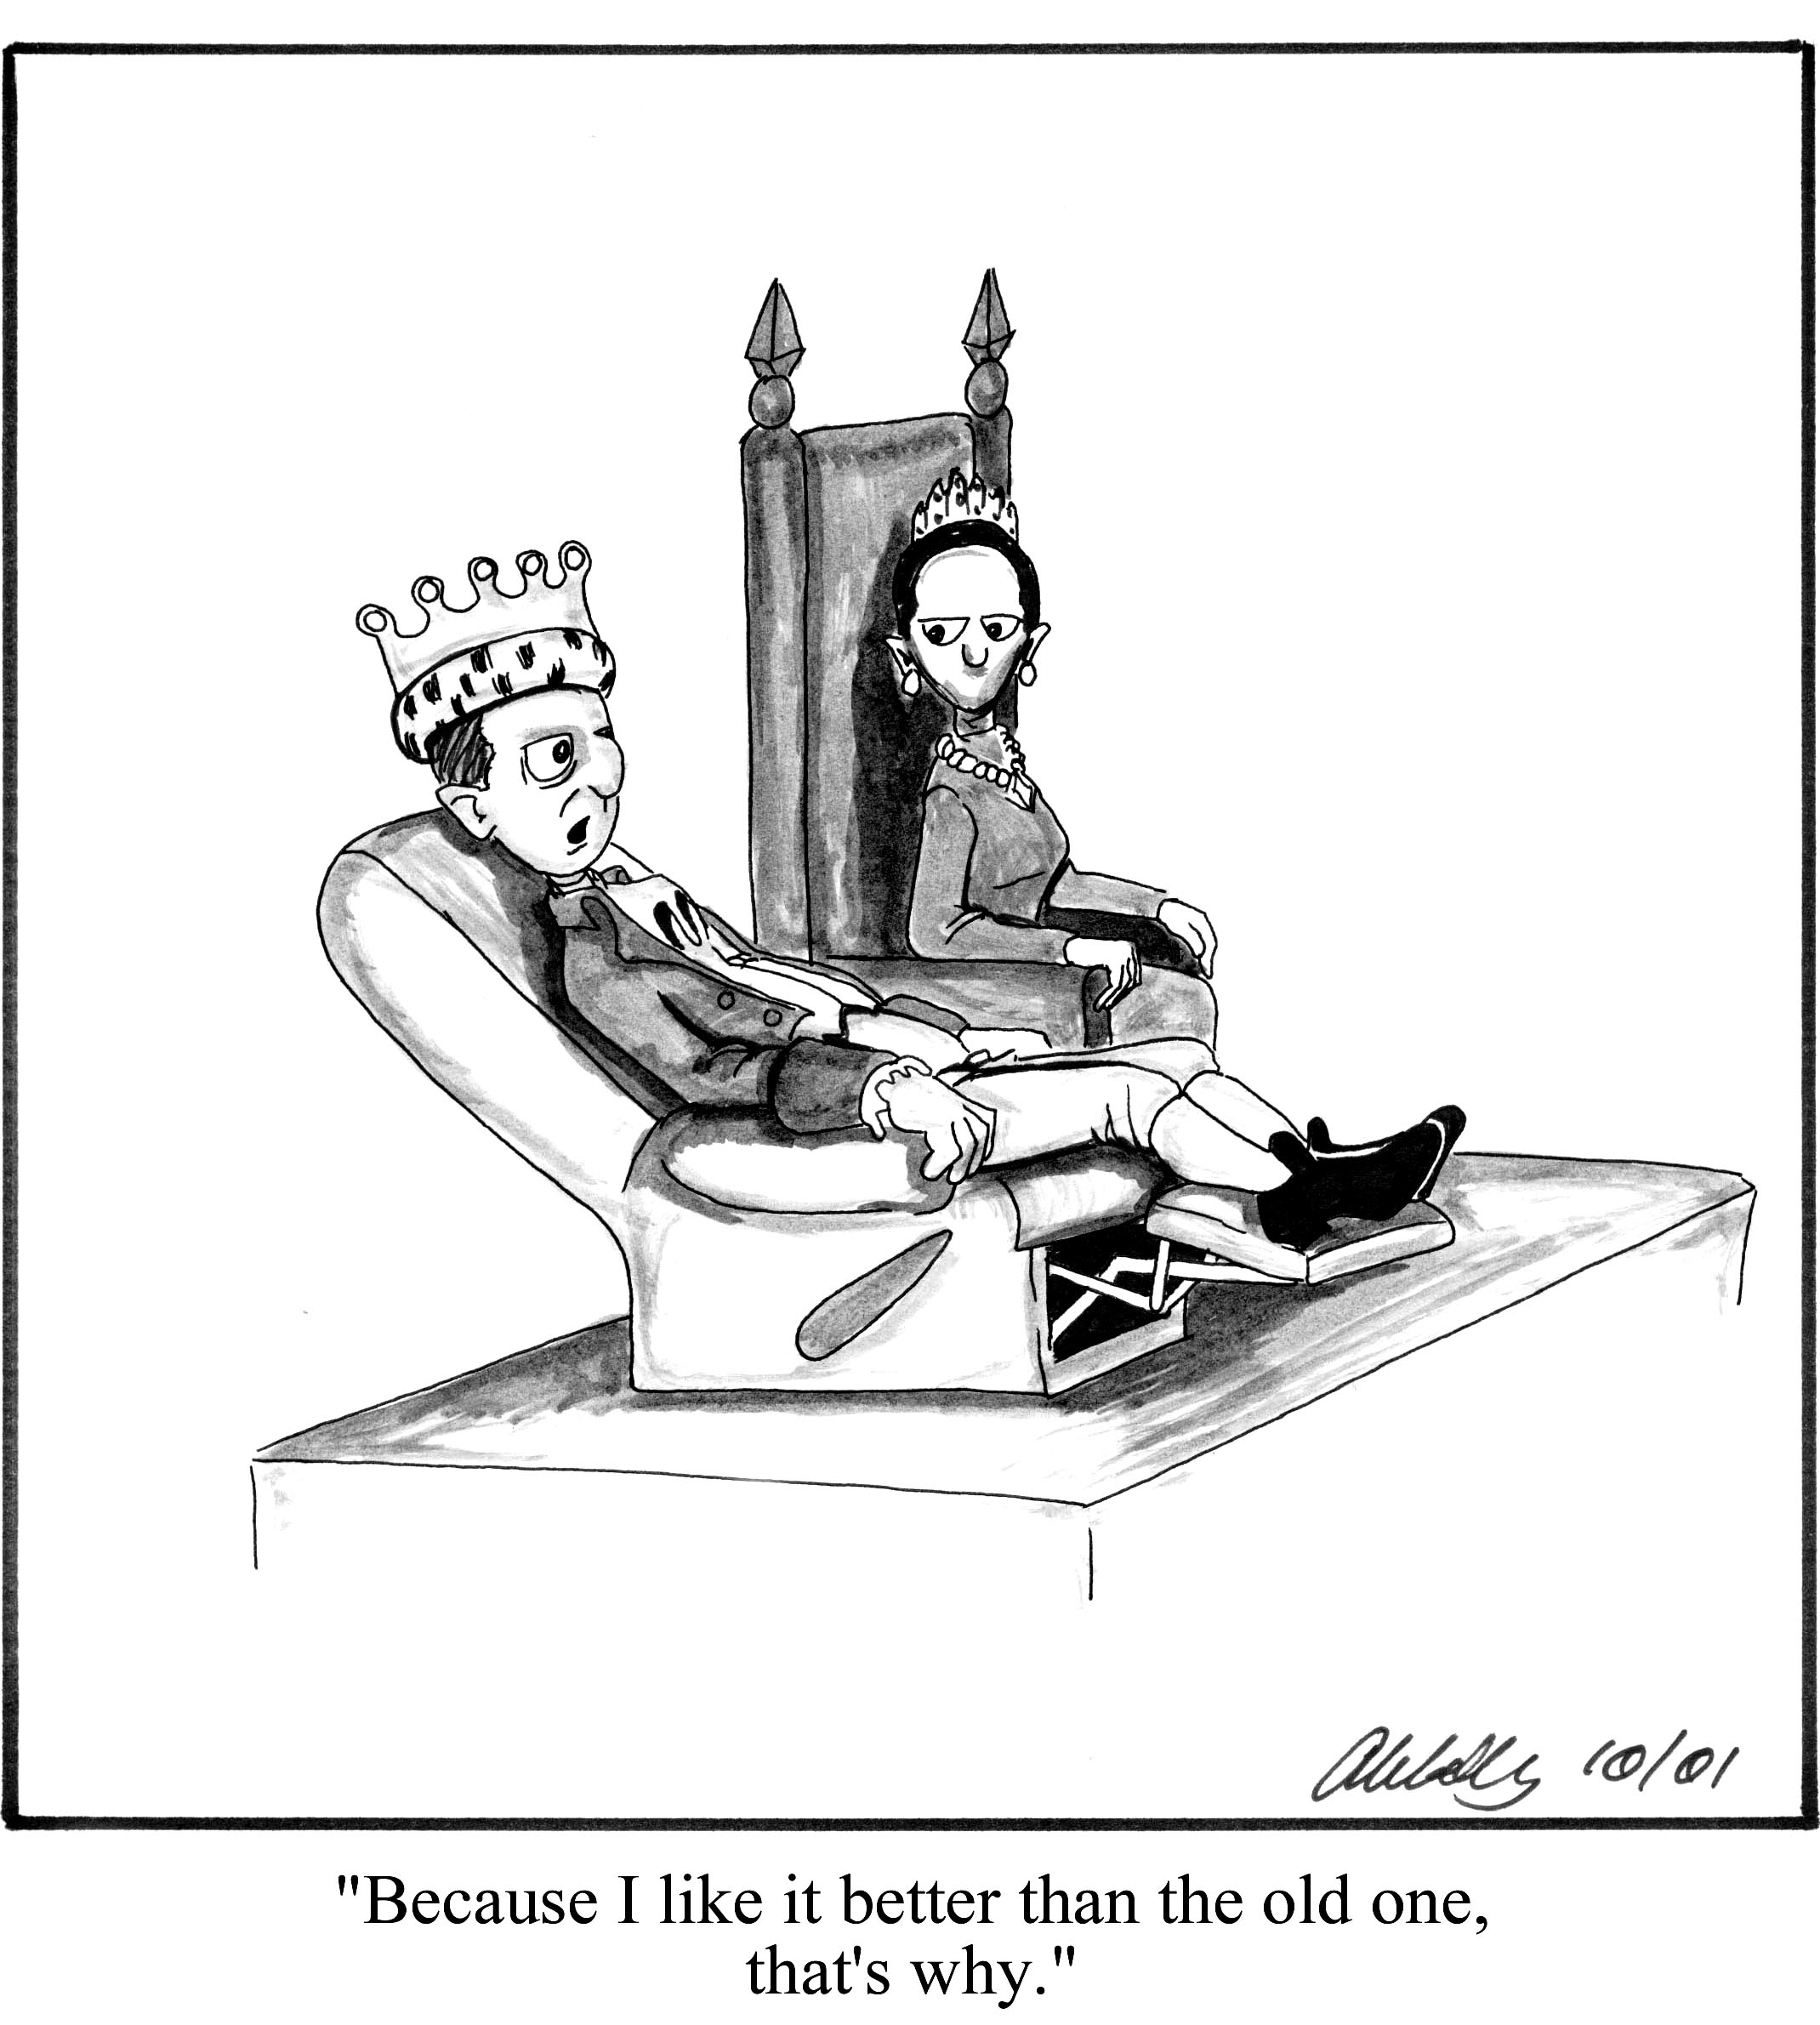
\includegraphics[width=0.5\textwidth]{throneEC.jpg}
  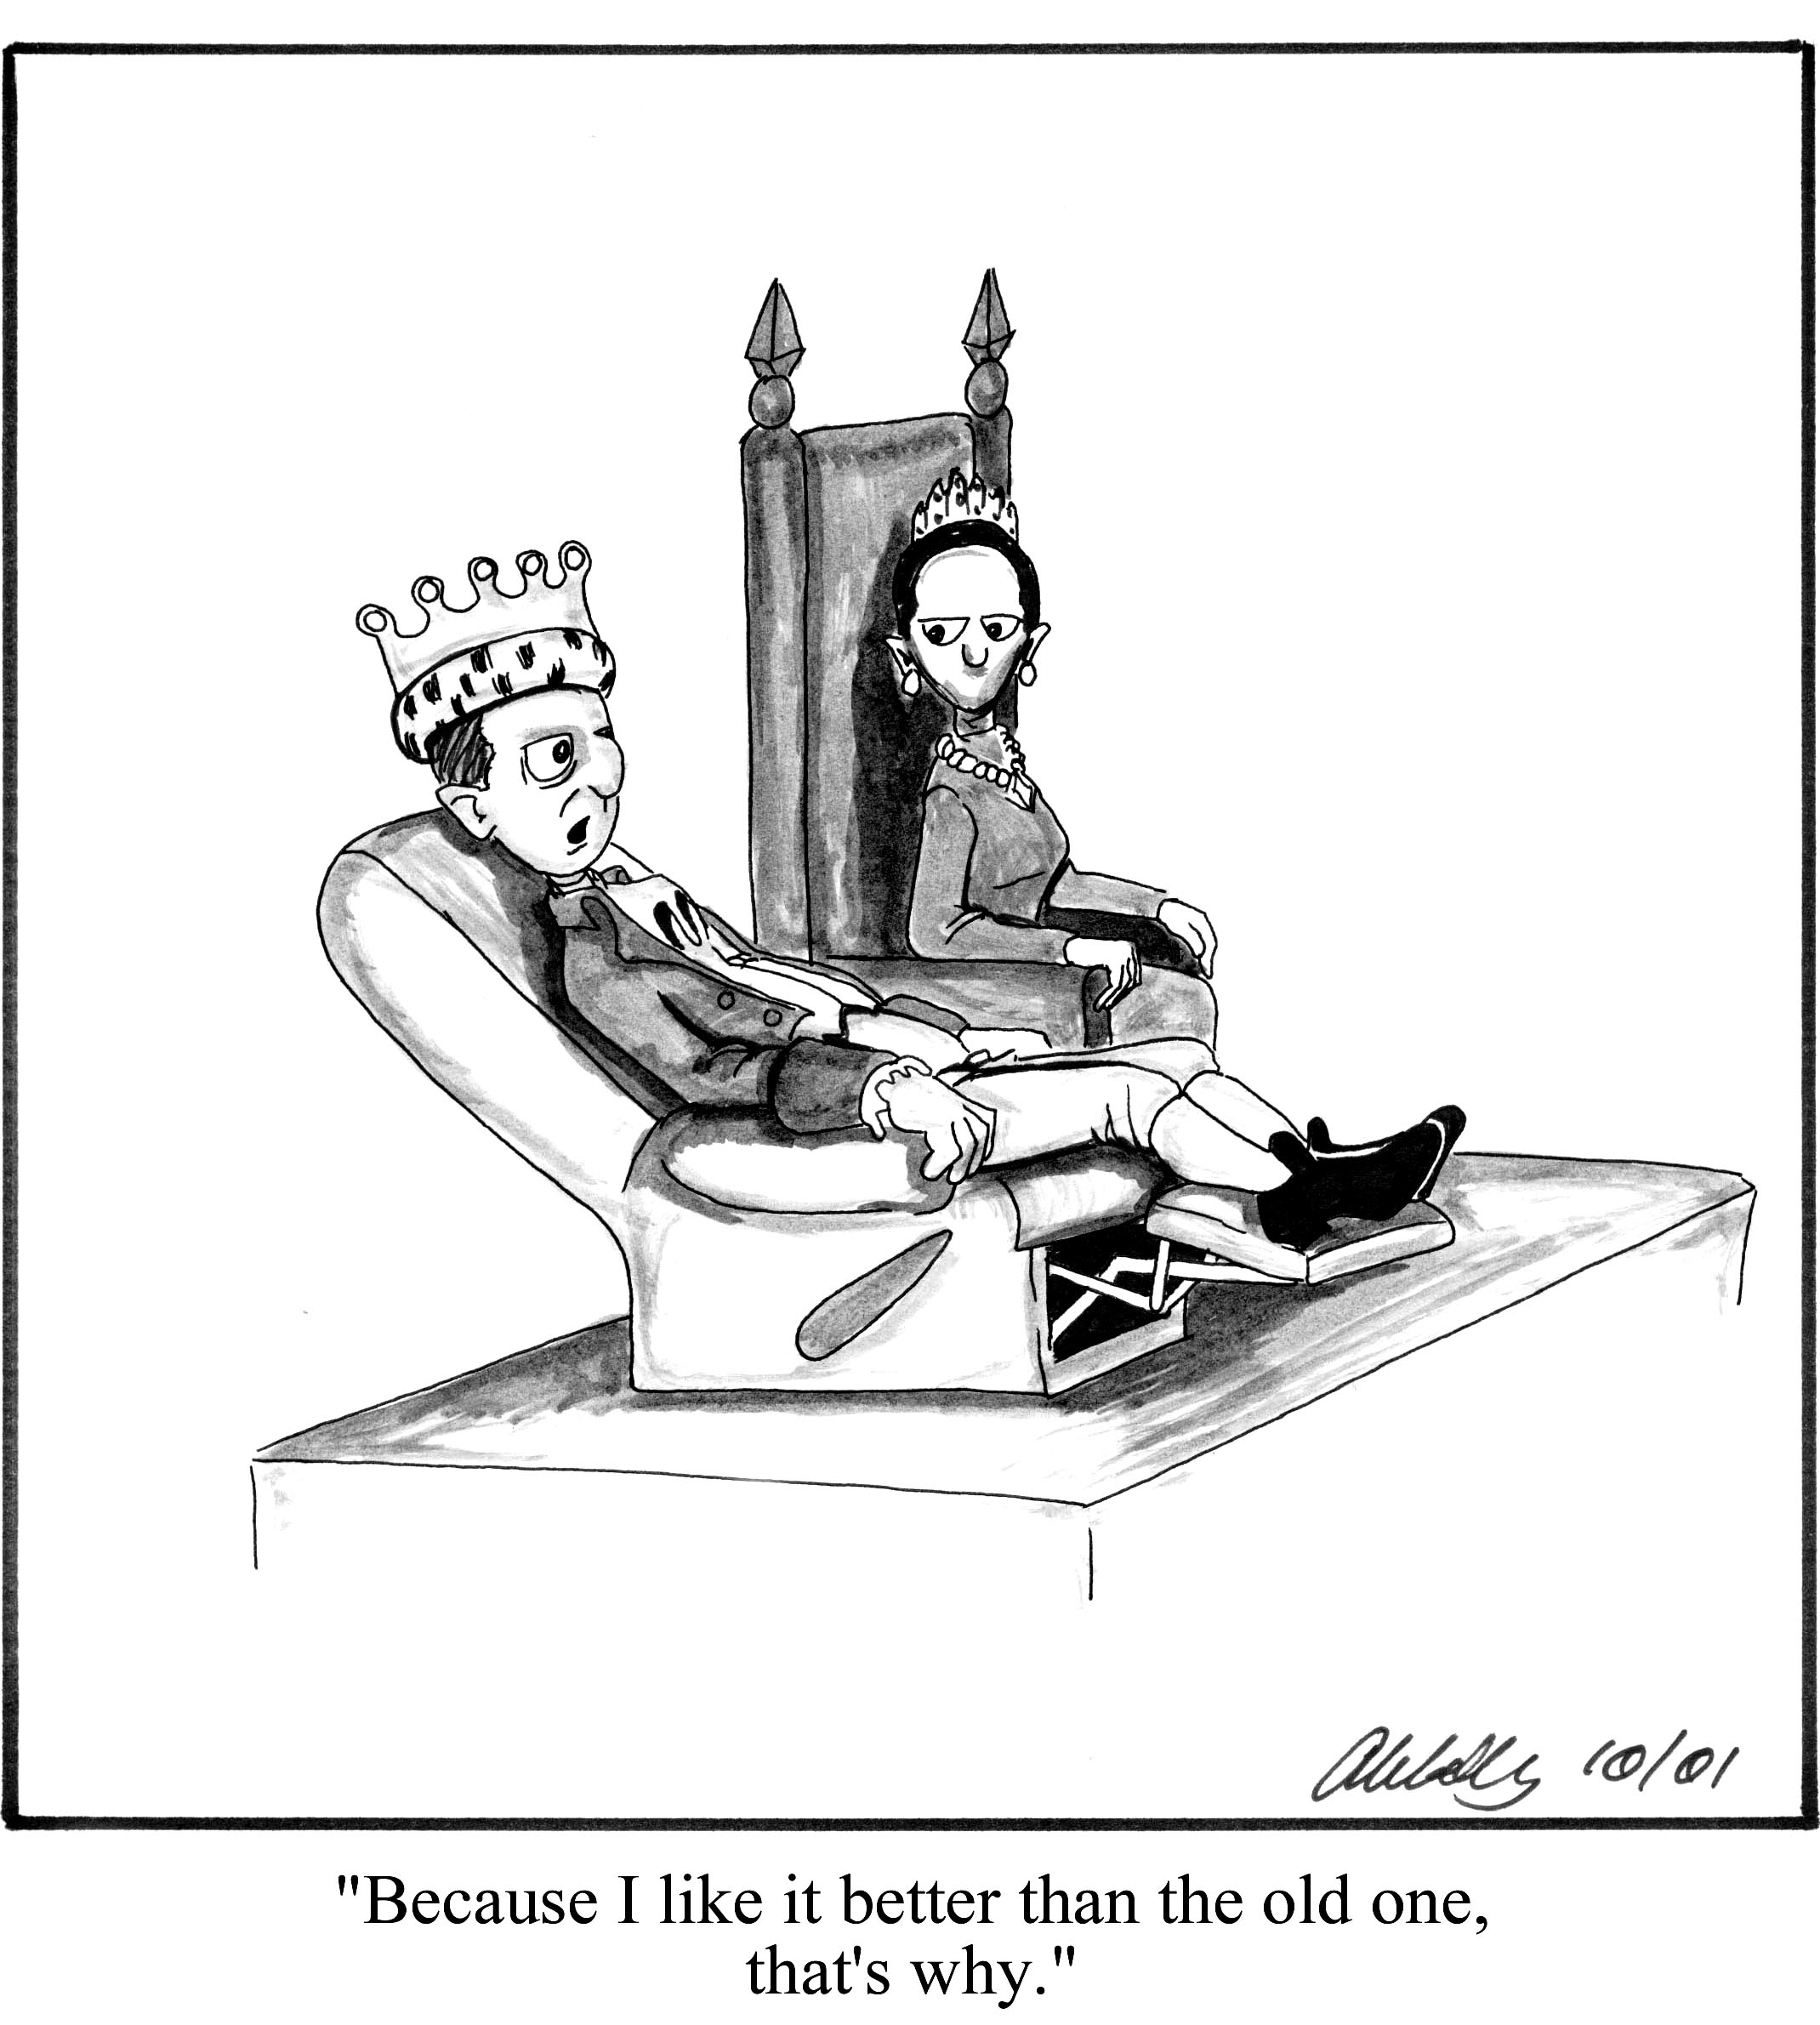
\includegraphics[width=0.3\textwidth]{throneEC.jpg}
  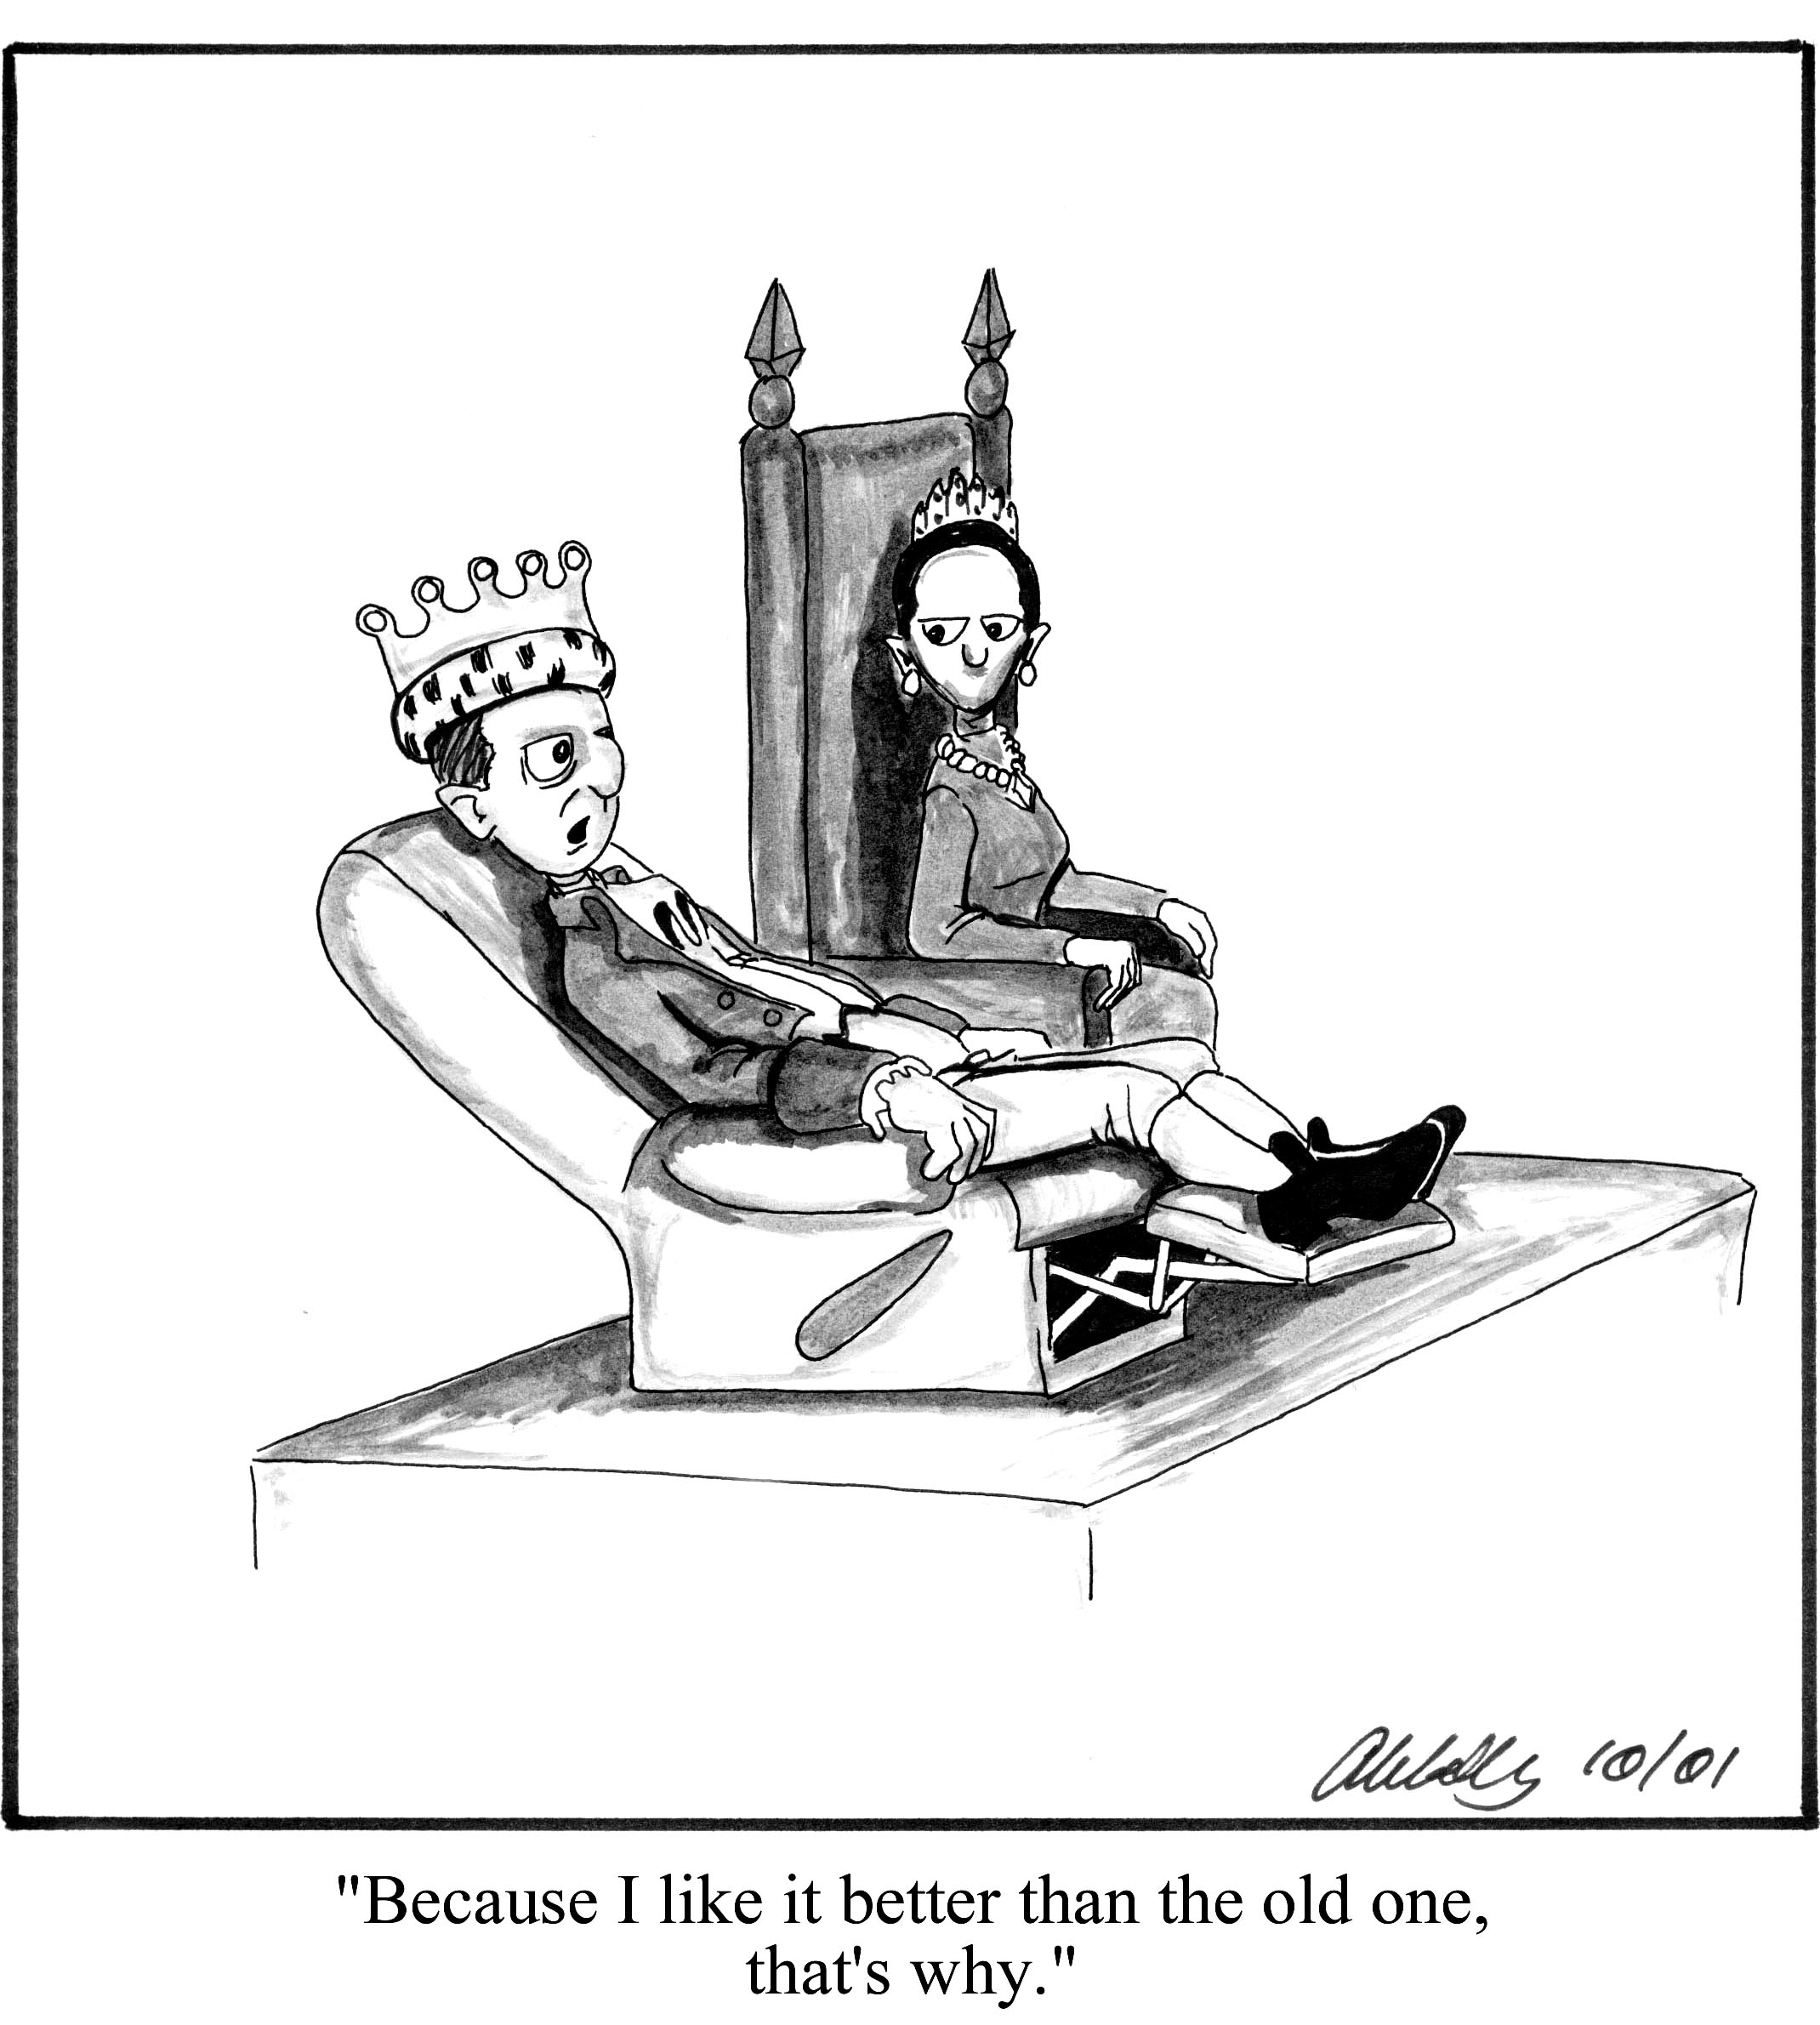
\includegraphics[width=0.15\textwidth]{throneEC.jpg}
\end{verbatim}

\subsection{A Universal Recipe}

\LaTeX\ has a very powerful weapon for reducing the size of almost
anythings. More precisely, it can reduce anything producing what
\LaTeX\ considers a box. This weapon is called
\verb|\scalebox|. Consider an example (check the source of this file
to see how it was produced).

\begin{center}
\begin{tabular}{|c|c|}
\hline \Huge
\begin{tabular}[b]{cr}
year & users \\ \hline
2007 &    47,753 \\
 2008 &    114,494 \\
 2009 &    207,506 \\
 2010 &   371,054 \\
\end{tabular}
&
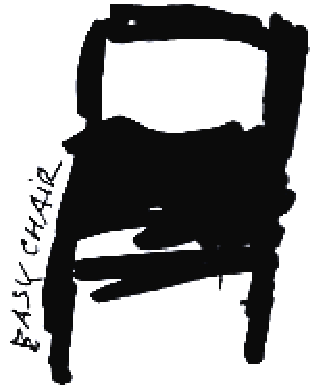
\includegraphics[width=0.28\textwidth]{chairEC}\\
\hline
\multicolumn{2}{|c|}{The number of users of EasyChair and one of its
  logos,}\\
\multicolumn{2}{|c|}{scaled to the number of users in 2010} \\
\hline
\end{tabular}
\end{center}
This is what happens when we put (almost) the same \LaTeX\ code in 
\verb|\scalebox{0.55923}{...}| to scale it down to the number of users
in 2009:

\begin{center}
\scalebox{0.55923}{%
\begin{tabular}{|c|c|}
\hline \Huge
\begin{tabular}[b]{cr}
year & users \\ \hline
2007 &    47,753 \\
 2008 &    114,494 \\
 2009 &    207,506 \\
 2010 &   371,054 \\
\end{tabular}
&
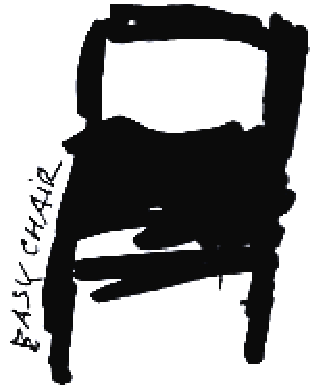
\includegraphics[width=0.28\textwidth]{chairEC}\\
\hline
\multicolumn{2}{|c|}{The number of users of EasyChair and one of its
  logos,}\\
\multicolumn{2}{|c|}{scaled to the number of users in 2009} \\
\hline
\end{tabular}}
\end{center}
We can scale it down even further to the 2008 figure using
\verb|\scalebox{0.30856}{...}|:

\begin{center}
\scalebox{0.30856}{%
\begin{tabular}{|c|c|}
\hline \Huge
\begin{tabular}[b]{cr}
year & users \\ \hline
2007 &    47,753 \\
 2008 &    114,494 \\
 2009 &    207,506 \\
 2010 &   371,054 \\
\end{tabular}
&
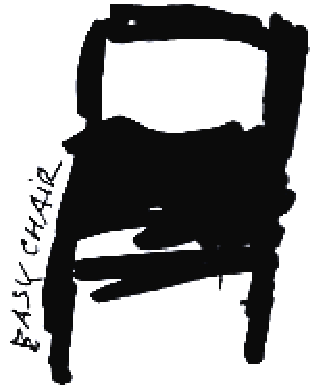
\includegraphics[width=0.28\textwidth]{chairEC}\\
\hline
\multicolumn{2}{|c|}{The number of users of EasyChair and one of its
  logos,}\\
\multicolumn{2}{|c|}{scaled to the number of users in 2008} \\
\hline
\end{tabular}}
\end{center}
or further down to 2007:

\begin{center}
\scalebox{0.12870}{%
\begin{tabular}{|c|c|}
\hline \Huge
\begin{tabular}[b]{cr}
year & users \\ \hline
2007 &    47,753 \\
 2008 &    114,494 \\
 2009 &    207,506 \\
 2010 &   371,054 \\
\end{tabular}
&
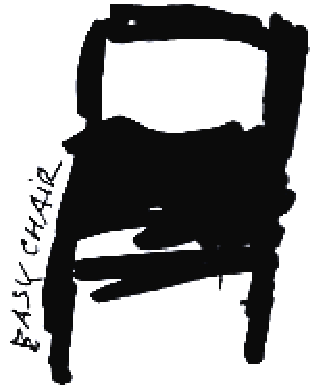
\includegraphics[width=0.28\textwidth]{chairEC}\\
\hline
\multicolumn{2}{|c|}{The number of users of EasyChair and one of its
  logos,}\\
\multicolumn{2}{|c|}{scaled to the number of users in 2008} \\
\hline
\end{tabular}}
\end{center}

This size reduction technique is very efficient: using the right scale
you may post your whole article on Twitter in a single tweet. However,
it may also may parts of your text virtually unreadable with an
unfortunate side effect of annoying reviewers. 

\section{Submitting Your Article Through EasyChair}

This section is intended only for the authors and editors of EasyChair
proceedings and Procedia volumes. 

When you prepare an article for either of these, it should be
submitted through EasyChair. EasyChair automates the submission
process as much as possible and goes to a great length to ensure that
your article can be published and printed. Publication for EasyChair
means much more than just putting a PDF of your article online. It
collects a some meta-information about the article to classify it,
find similar articles, make it easily searchable, and index it in
various Web services, such as DBLP. This section explains how
EasyChair processes your article. 

\subsection{Submitting the Article}

Submitting the article is easy. All you should do is to put the source
of your article in a single zip file. The source must contain all
auxiliary files required to create a PDF file of your article: this
includes images, bibliography, and all non-standard \LaTeX\ packages
you used\footnote{ 
  A non-standard \LaTeX\ package is a package that is not included in
  CTAN. 
} For example, suppose that your main \LaTeX\ file is
\texttt{main.tex}, it inputs another file \texttt{macros.tex} and uses
the file \texttt{biblio.bib} to produce the bibliography. Suppose it
also uses two images \texttt{images/easy.jpg} and
\texttt{images/easy.jpg}. Then you should create a zip archive
containing all these files. Suppose all these files are put in a
directory \texttt{mypaper} on your computer, where \texttt{images} is
a subdirectory of \texttt{mypaper}

On almost any operating system (Linux,
Windows, or Mac) you can achieve this by using the following sequence
of commands:

\begin{verbatim}
cd mypaper
zip -r mypaper.zip *
\end{verbatim}
This will create a zip archive \texttt{mypaper.zip} including all
files in the directory \texttt{mypaper} and its subdirectories. 

\subsection{EPiC Series and Kalpa Publications}
\label{subsec:EPiC}

If you publish your article in the EasyChair EPiC series, our aim is to produce
a nicely looking EPiC Series header, see Figure~\ref{fig:epicheader} on page
\pageref{fig:epicheader} for an idea. The images and information in the header
will be added by EasyChair automatically and depend on the subseries and the
volume information.

\begin{figure}
  \begin{centering}
    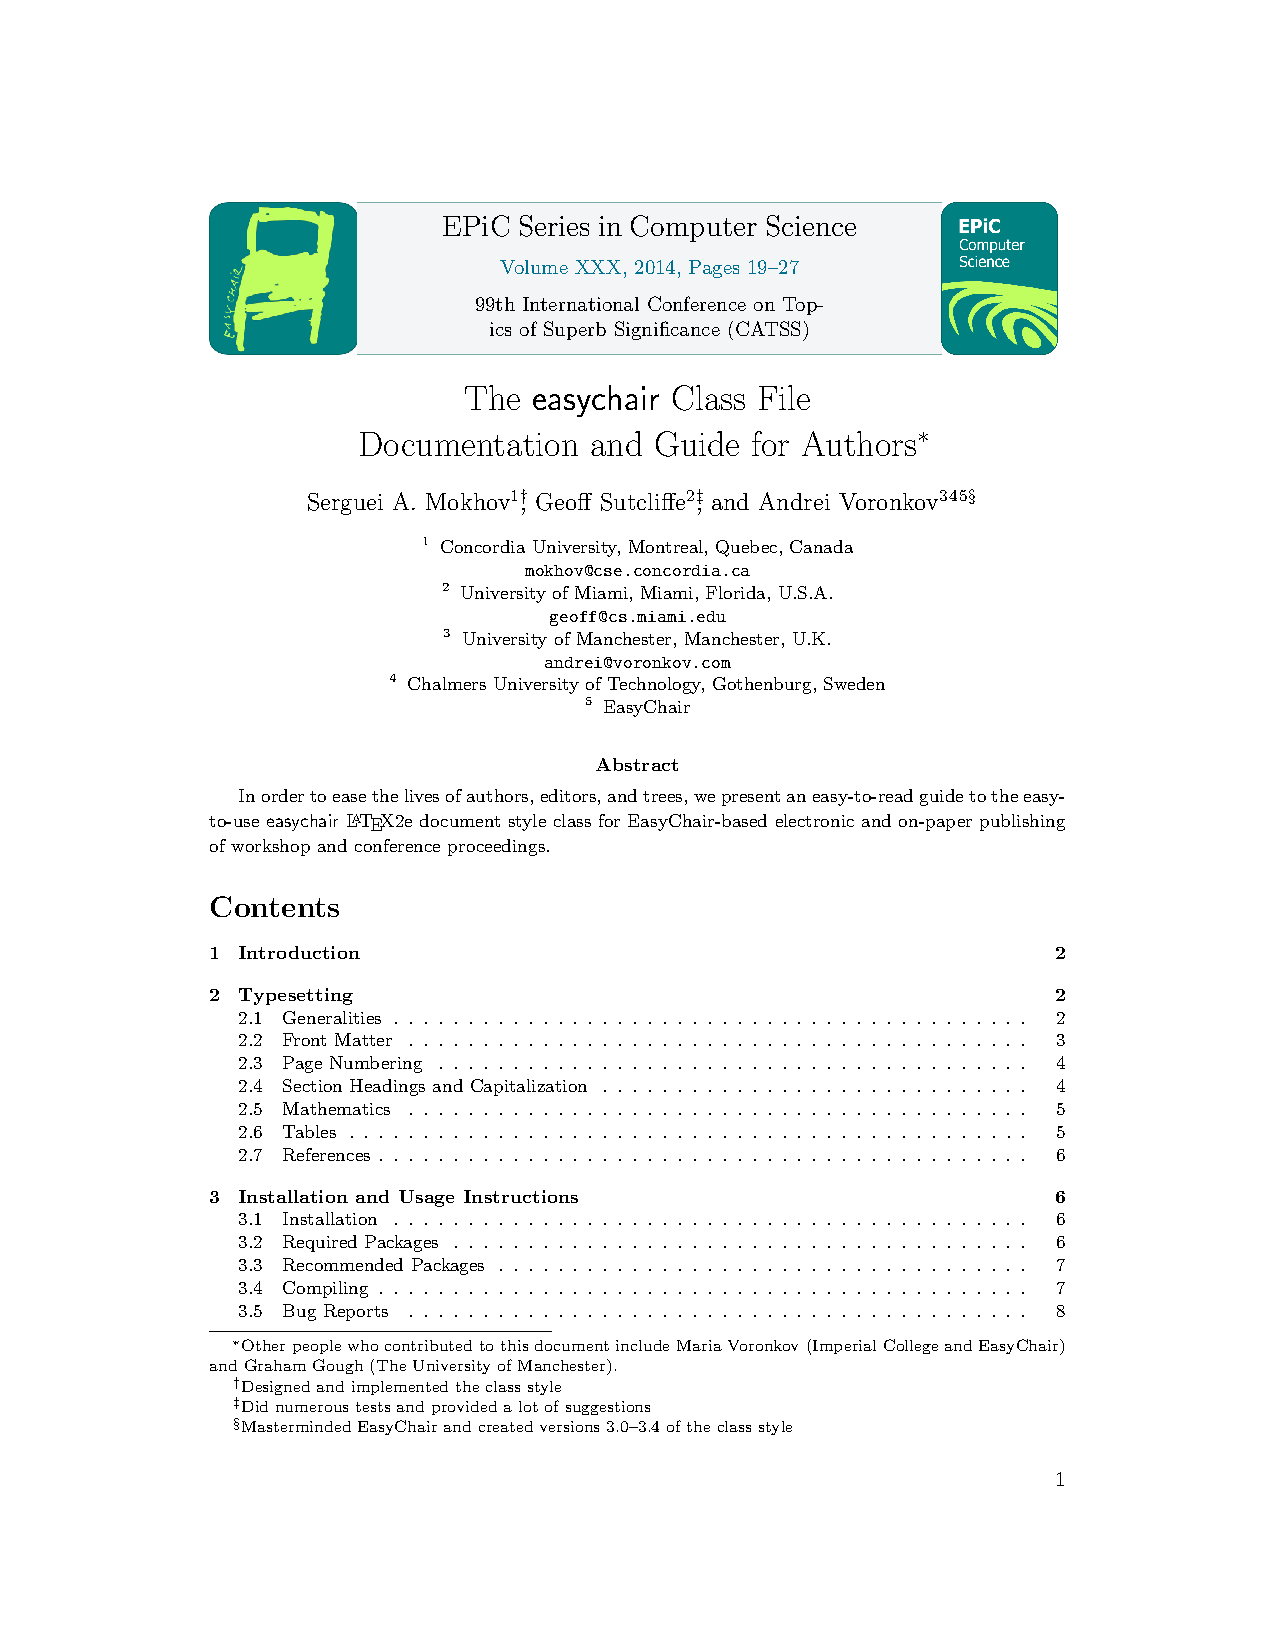
\includegraphics[width=0.89\textwidth]{epic.pdf}
    \caption{This document with an EPiC Series header} 
    \label{fig:epicheader}
  \end{centering}
\end{figure}

To ensure that the layout of your document will not change when the header is
added, you should use the option \texttt{EPiC} as follows:

\small
\begin{verbatim}
\documentclass[EPiC]{easychair}
\end{verbatim}
\normalsize
This will reserve space for the header on the top of the first page of your
article. 

%------------------------------------------------------------------------------
\section{Future Work}
\label{sect:future-work}

We plan to further strengthen the {\easychair} class and promote it for 
electronic publishing for EasyChair-powered conferences and workshops,
and take over the world, as shown in Figure~\ref{fig:easythrone}. We
aim at creating a new model of \emph{affordable publishing}, where
anybody can become a low-cost publisher. The
\href{http://www.easychair.org/publications/EPiC}{EasyChair EPiC
  Series} and
the
\href{http://www.easychair.org/publications/Kalpa}{EasyChair Kalpa Publications} 
are our first contributions to affordable open access publishing.

\begin{figure}[tb]
  \begin{centering}
    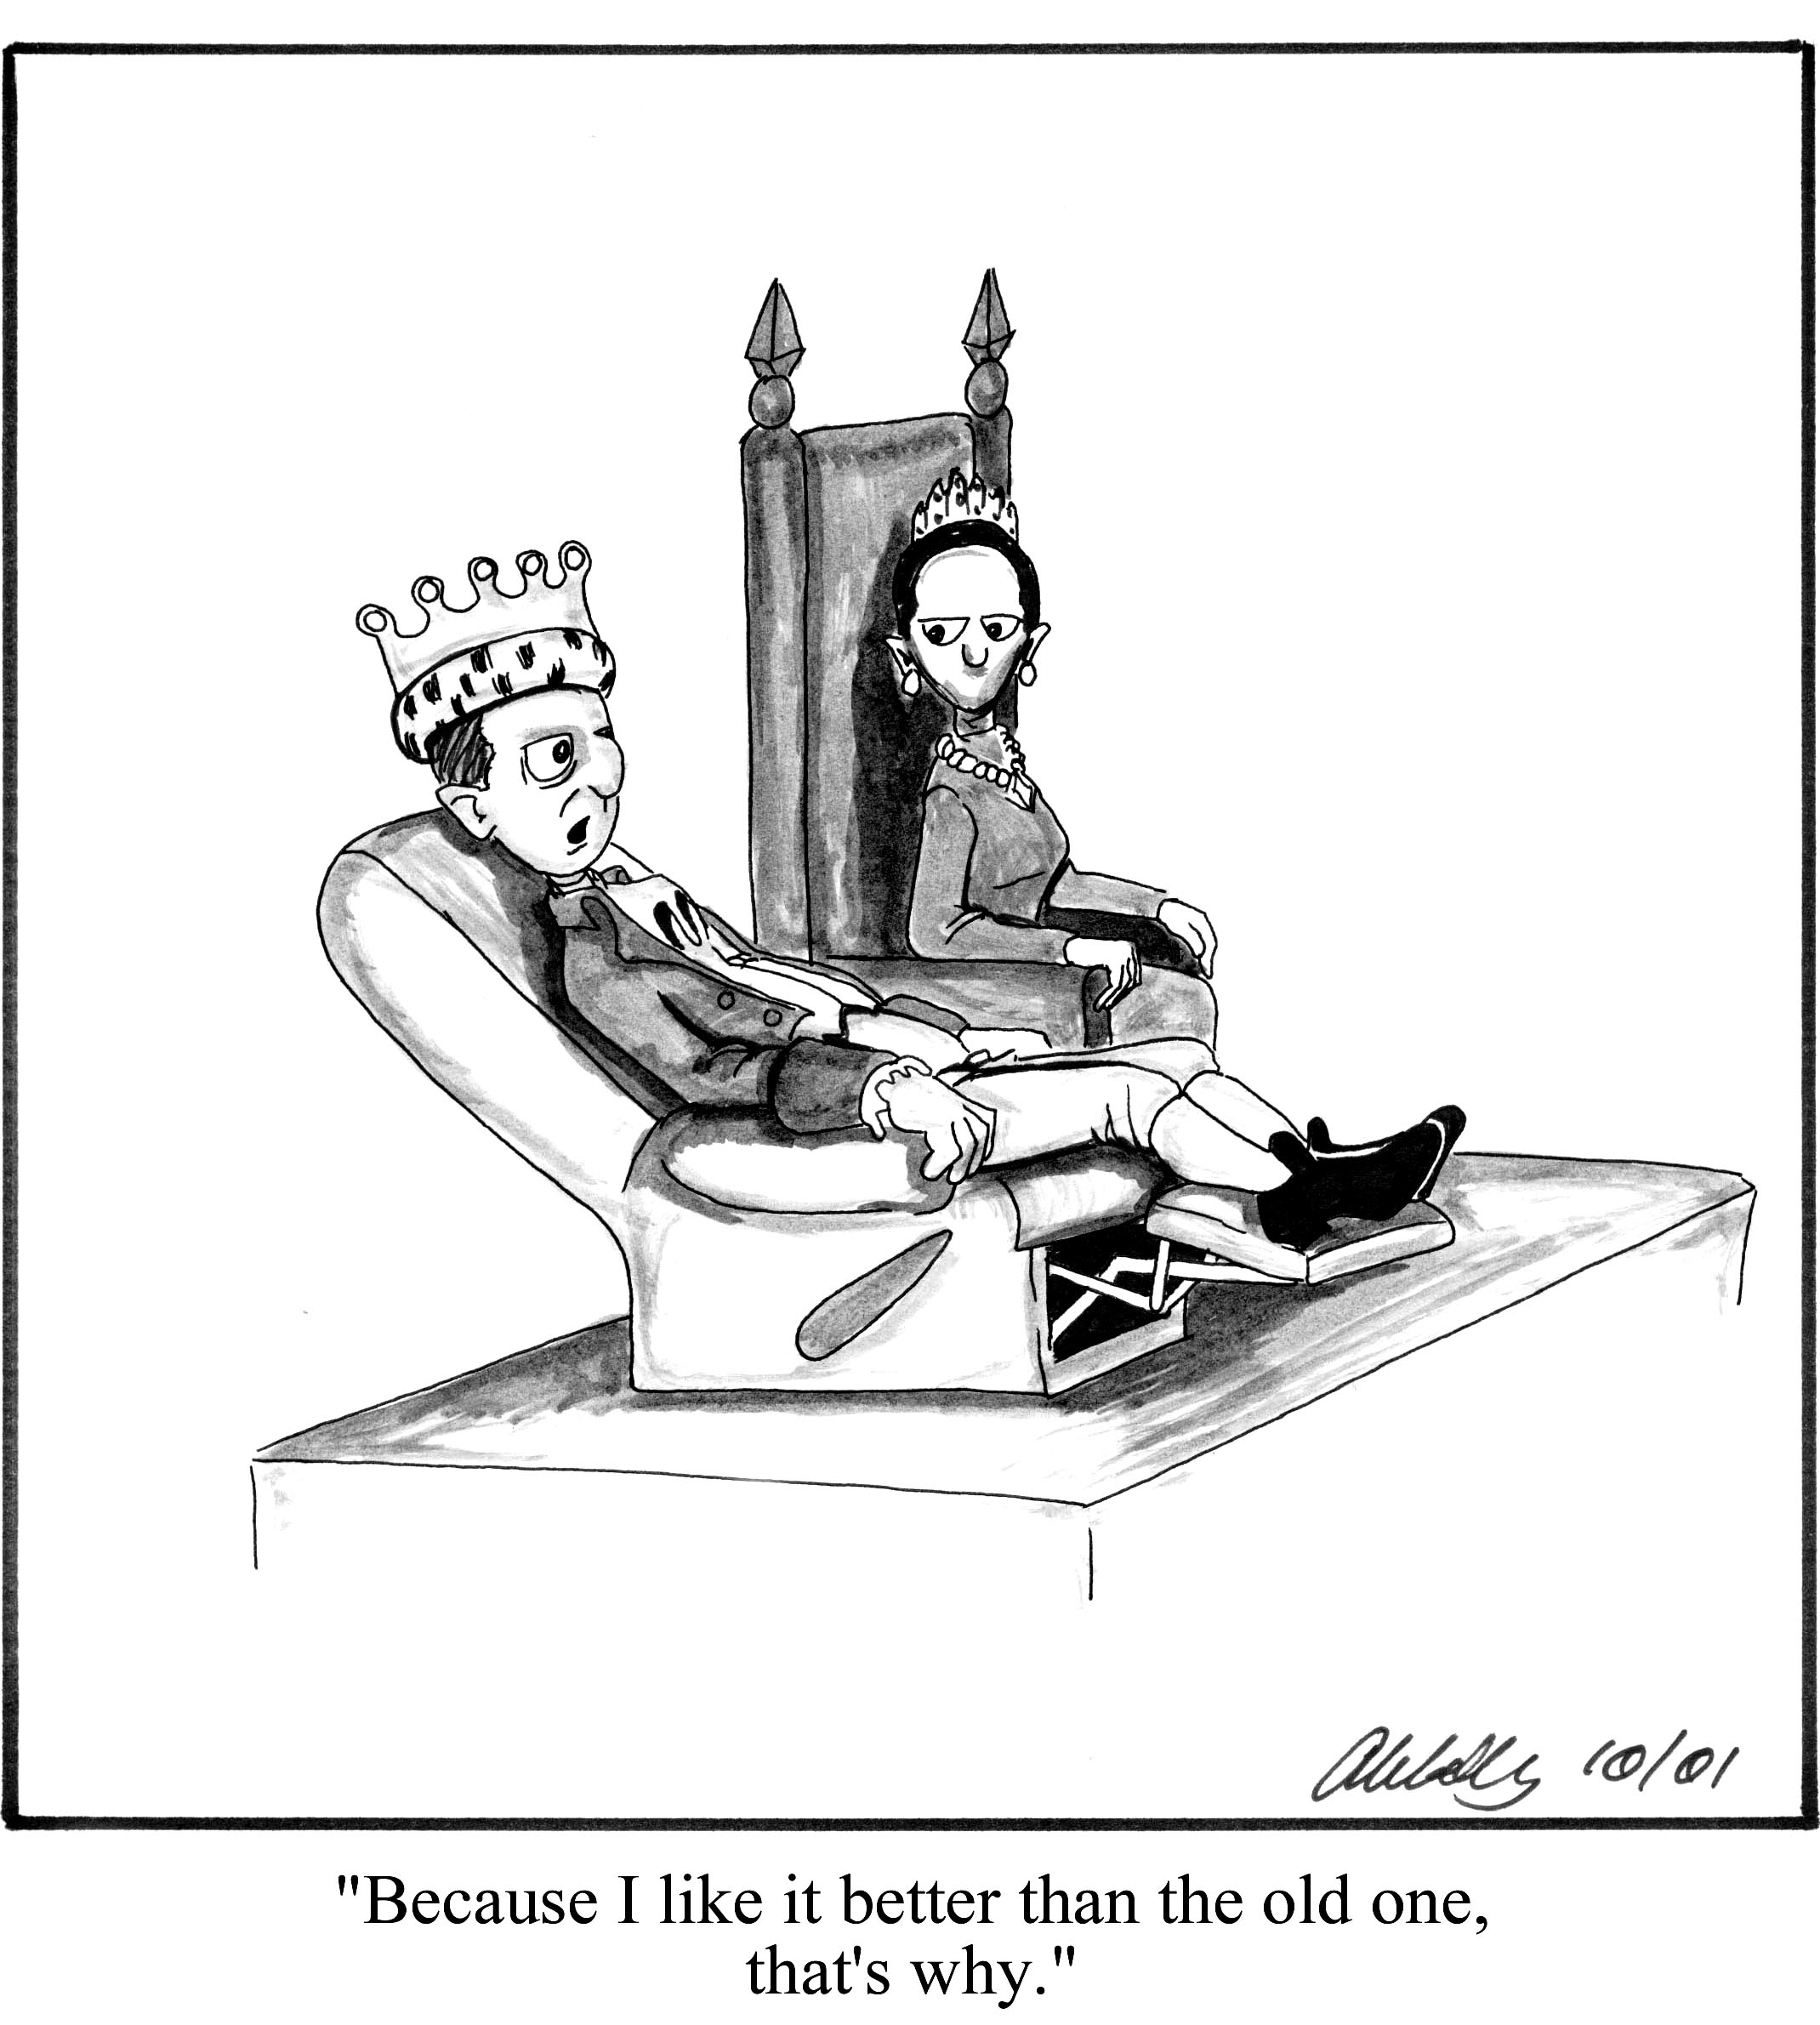
\includegraphics[width=0.5\textwidth]{throneEC.jpg}
    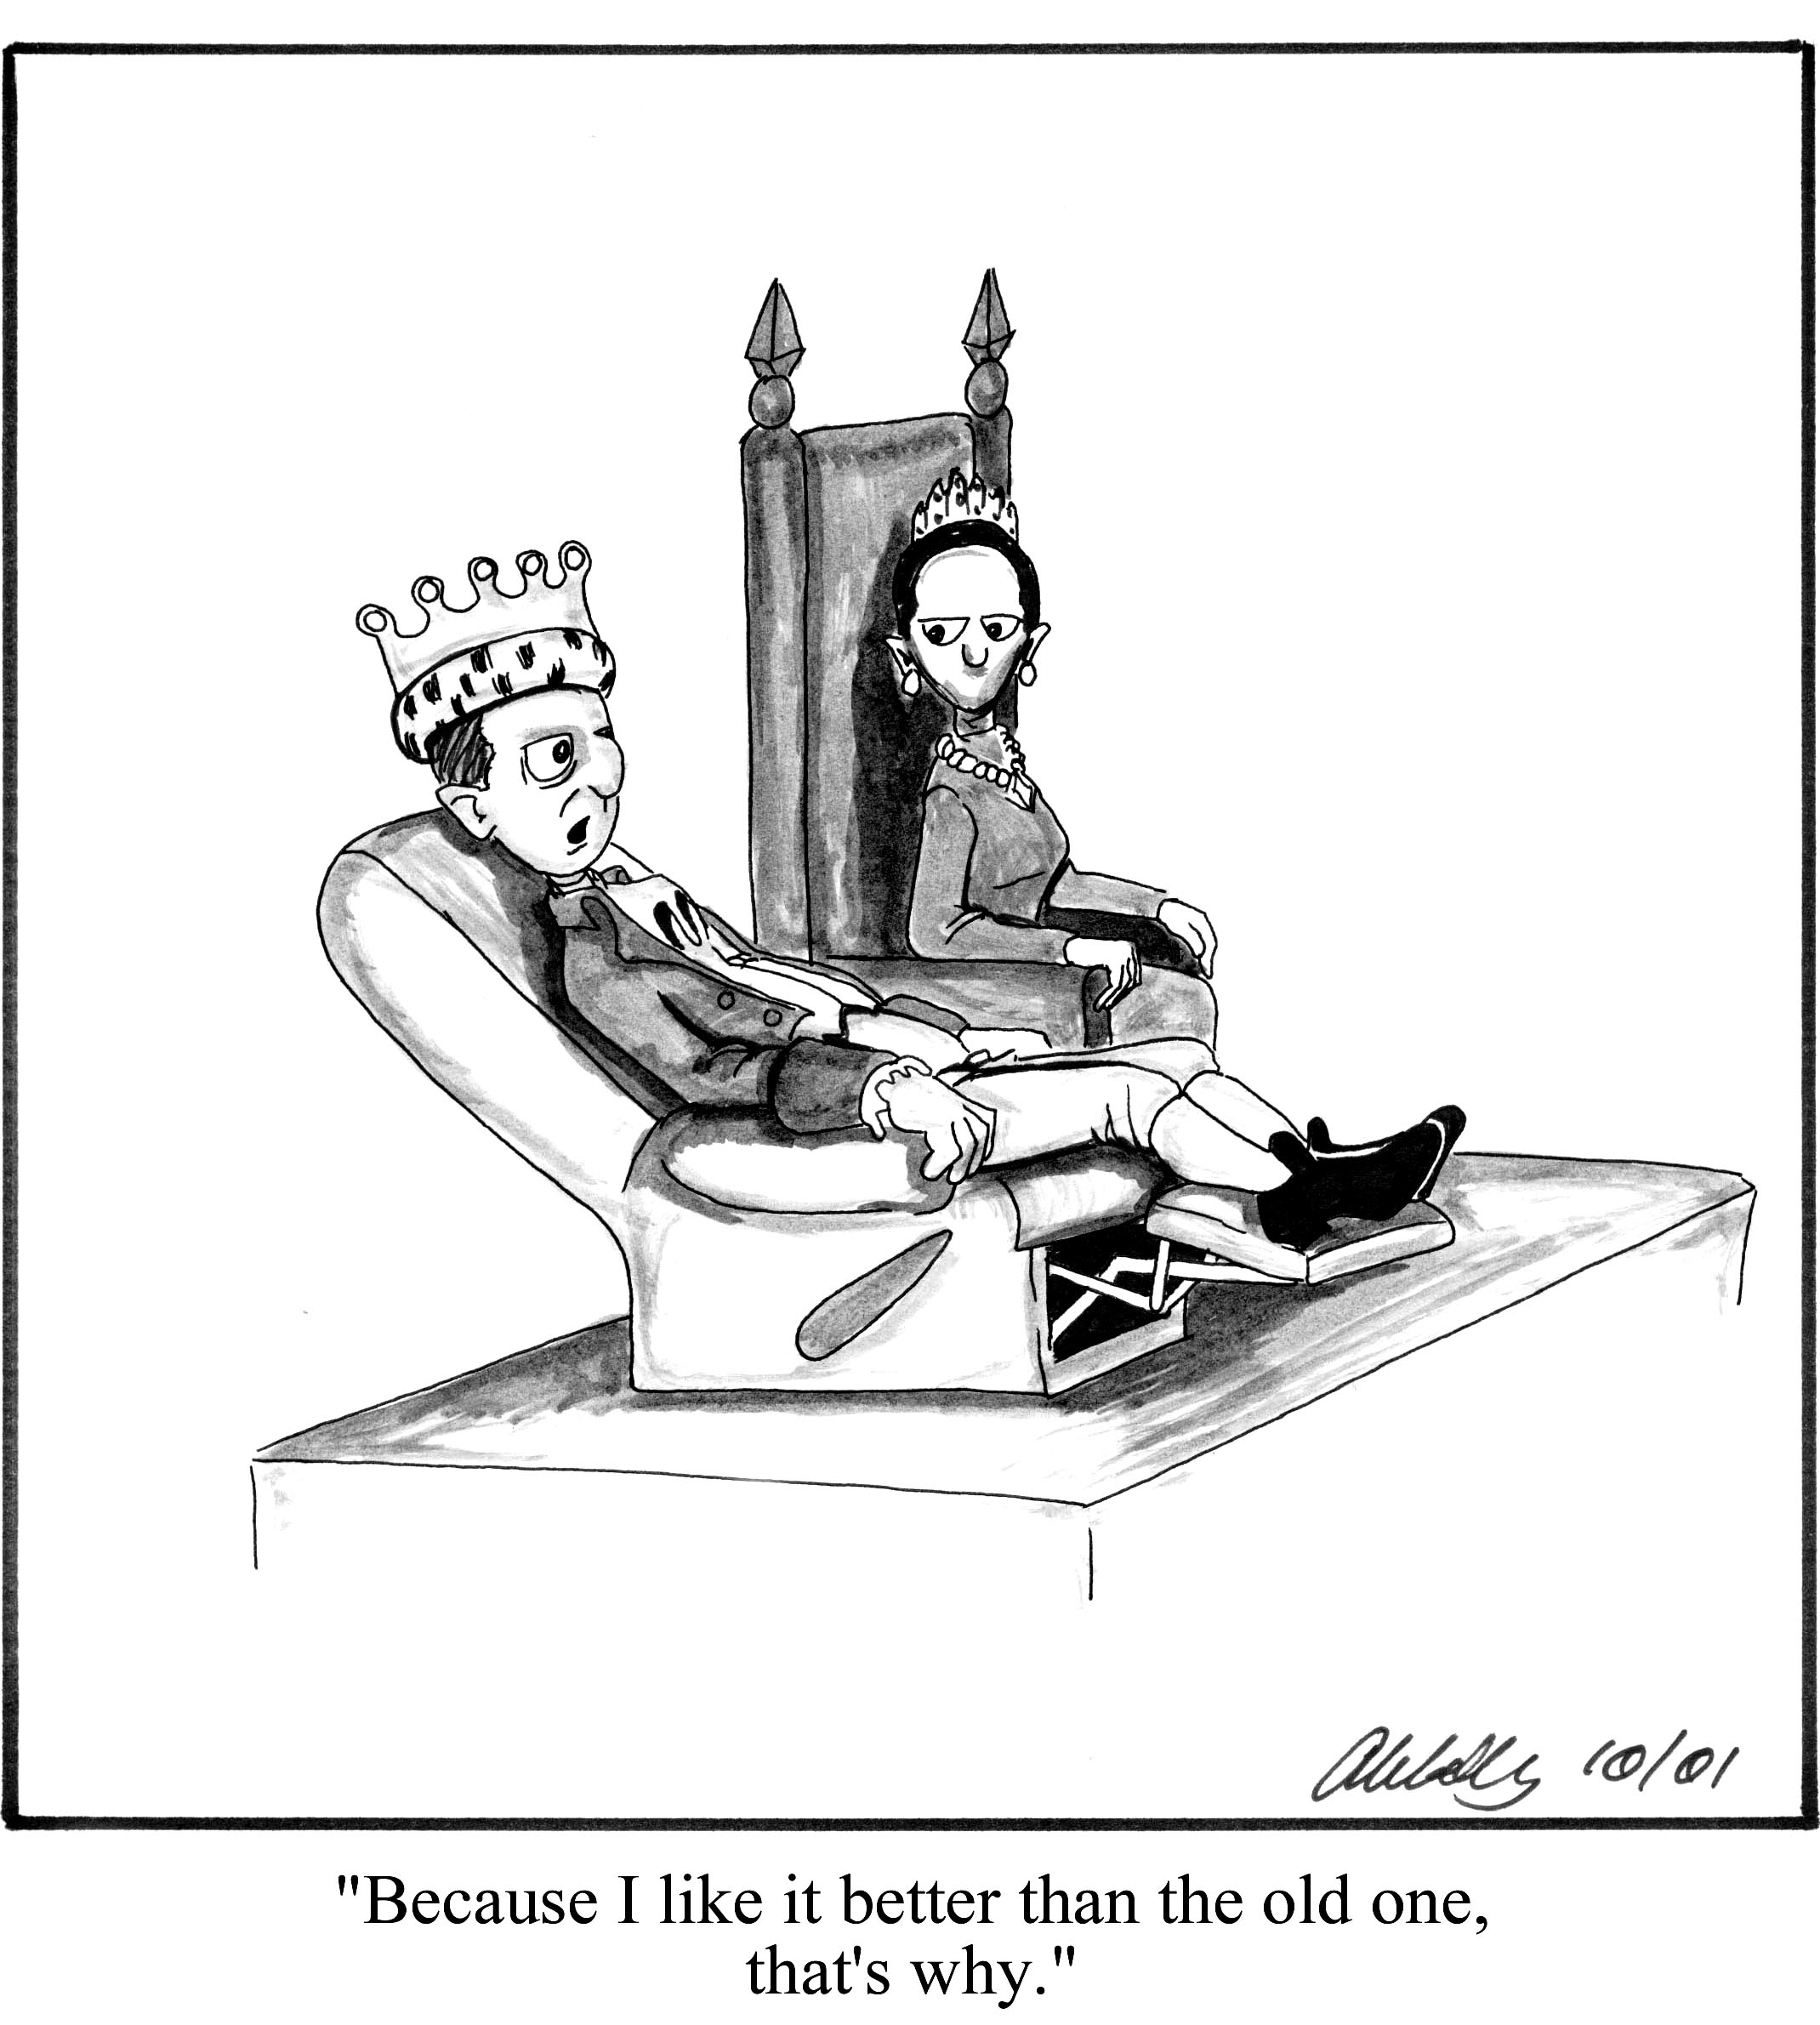
\includegraphics[width=0.3\textwidth]{throneEC.jpg}
    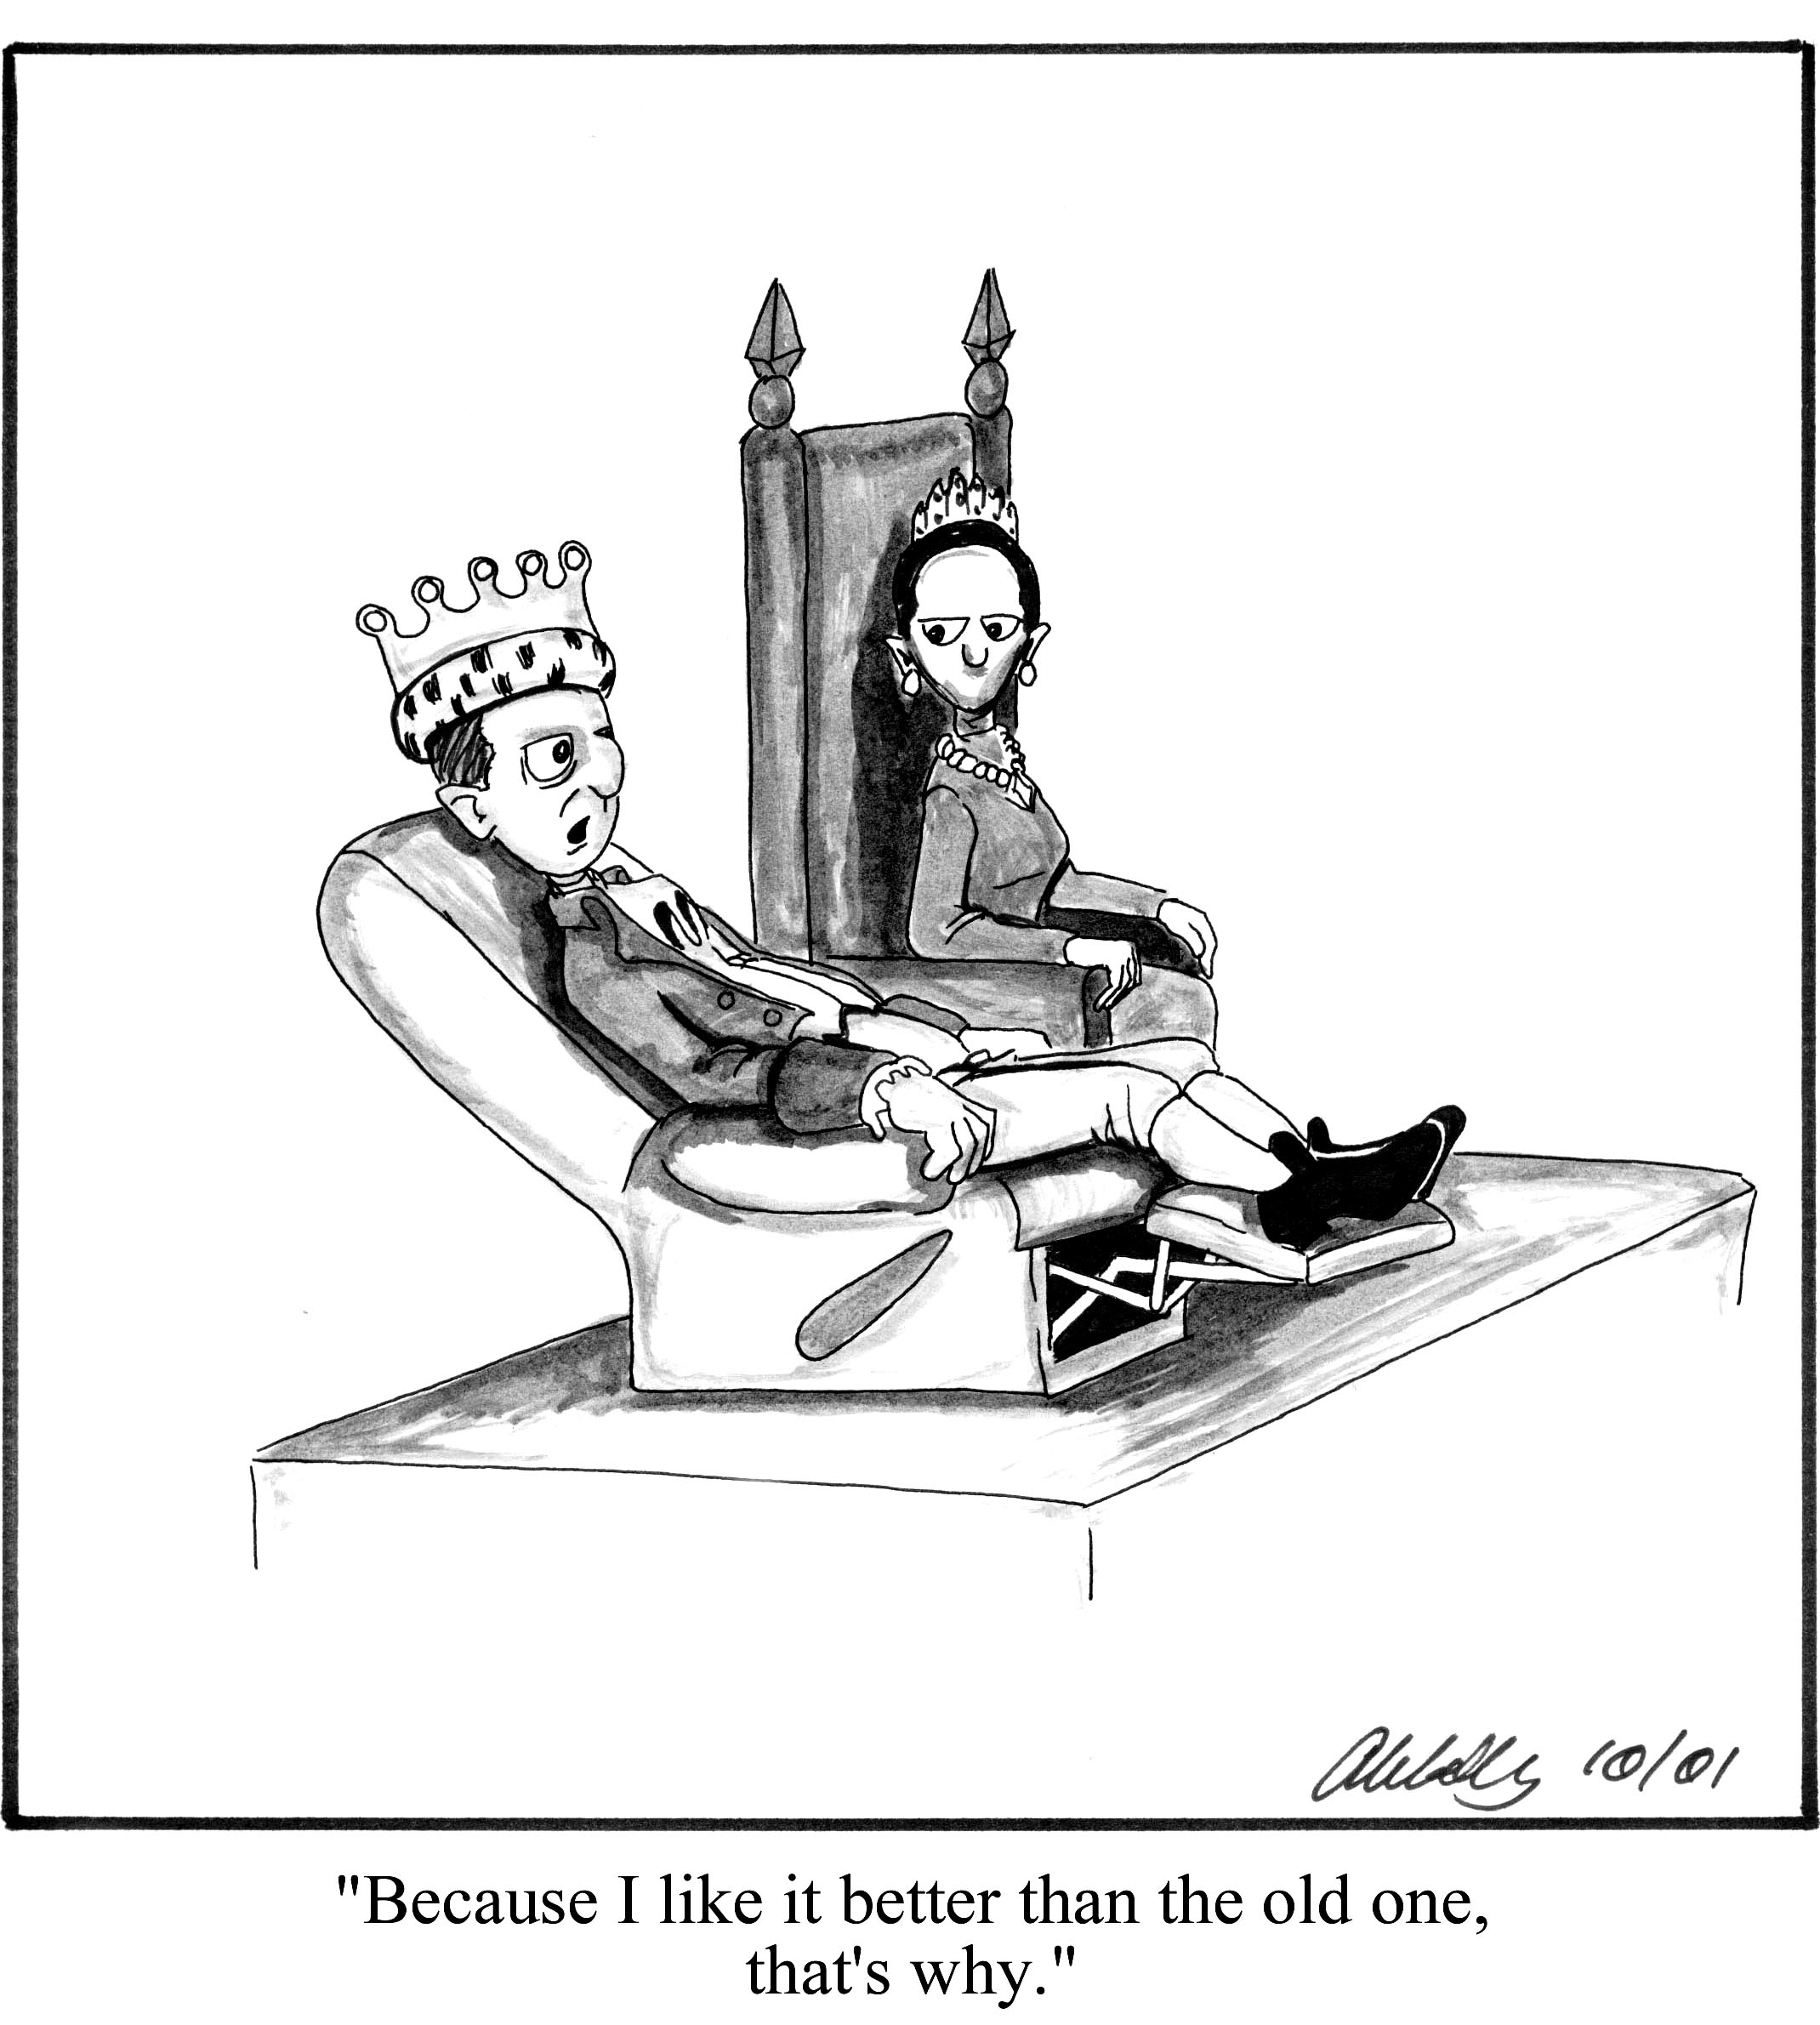
\includegraphics[width=0.15\textwidth]{throneEC.jpg}
  \end{centering}
  \caption{Why one should use EasyChair}
  \label{fig:easythrone}
\end{figure}

%------------------------------------------------------------------------------
\section{Acknowledgments}
\label{sect:acks}

\begin{itemize}
\item
Aleksander Kosenkov for the graphics that are used here and on the EasyChair 
website~\cite{easychair}.

\item
Graham Gough (The University of Manchester) for implementing title-related
commands.

\item
Thomas F. Sturm (Universit\"at der Bundeswehr M\"unchen) for implementing the
\LaTeX\ part of the headers used for the EasyChair EPiC series.

\item
The CTAN \cite{ctan} and {\LaTeX} communities \cite{texniccenter,miktex}.

\item
Guilin Qi, Jasmin Christian Blanchette, Leslie Lamport, Uwe Pfeiffer,
and others for constructive feedback on the style, most of which had been
incorporated in version 2 of the class style.
\end{itemize}

\label{sect:bib}
\bibliographystyle{plain}
%\bibliographystyle{alpha}
%\bibliographystyle{unsrt}
%\bibliographystyle{abbrv}
\bibliography{easychair}

%------------------------------------------------------------------------------
\appendix
\section{{\easychair} Requirements Specification}
\label{sect:easychair-requirements}

The following high-level requirements were set for the development of 
the {\easychair} class, and were refined as development went along.

\begin{enumerate}
\item
The style should be easy to use. 
The average {\LaTeX} user should not need to read a long manual.

\item
It should be economical in space but the text should be nice-to-read.

\item
It should use fonts producing a reasonable-quality PDF.

\item
The bibliography should produce hyperlinks.

\item
Sections should produce menu sections in PDF.

\item
The text should look good on both A4 and letter paper.

\item
The style should be single-column for convenience of scrolling.

\item
The print area should be convenient for printing using print-on-demand publishers.

\item
Running heads.
\end{enumerate}

%------------------------------------------------------------------------------
% Index
%\printindex

%------------------------------------------------------------------------------
\end{document}

